\chapter{HASIL DAN PEMBAHASAN}
\label{chap:hasilpembahasan}

% Ubah bagian-bagian berikut dengan isi dari hasil dan pembahasan

Bab ini akan membahas hasil dan analisa dari desain sistem yang sudah dibuat dan implementasinya. Pengujian terhadap hasil dibagi menjadi beberap bagian.

\section{Pengujian Performa antar \emph{Weight}}
\label{sec:ujiperforma}
Repositori YOLOv5 menyediakan beberapa \emph{checkpoint} atau \emph{weight} yang merupakan hasil training model YOLOv5 dari dataset COCO yang dimanfaatkan sebagai \emph{pretrained model}. Ekspektasi penggunaan pretrained model ini yaitu bobot yang dihasilkan akan memiliki performa yang lebih tinggi daripada melakukan training tanpa pretrained model sama sekali. \emph{COCO Dataset} ini memiliki 80 \emph{class} berbeda. Seperti disebutkan pada \ref{sec:pelabelandataset} yaitu untuk keperluan penelitian ini hanya memerlukan 2 kelas yaitu "no\textunderscore helmet" dan "with\textunderscore helmet". Pada bagian ini akan dipaparkan dan dibandingkan performa antara tiap bobot yang dihasilkan dengan model pretrained dan yang tidak menggunakan pretrained model.

\subsection{Pengujian Performa \emph{Weight} dari Hasil \emph{Pretrain} COCO Dataset}
\label{subsec:ujiperforma_coco}
Beberapa \emph{pretrained model} yang disedikana dari repositori YOLOv5 yaitu YOLOv5n, YOLOV5s, YOLOv5m, YOLOv5l,YOLOv5l, dan YOLOv5x. Selain beberapa model pretrained tersebut juga ada versi untuk ukuran gammbar 1280 yaitu seri YOLOv5n6 hingga YOLOv5l6. Pada penelitian ini hanya menggunakan variasi YOLOv5n hingga YOLOv5l karena variasi YOLOv5x dan versi seri 6 untuk ukuran gambar 1280 membutuhkan waktu yang lebih lama. Perbedaan - perbedaan yang ada pada bobot - bobot pretrained tersebut berasal dari konfigurasi awal dari training pada dataset COCO yang menggunakan YOLOv5, terutama pada paramter "depth\textunderscore multiple" dan "width\textunderscore multiple".
Proses validasi hasil training dilakukan menggunakan dataset Deteksi Helm Keselamatan Kerja yang pembagiannya dijelaskan pada bagian \ref{sec:preprocessing} yang berjumlah 1200 gambar dengan kelas "no\textunderscore helmet" berjumlah 1322 label dan kelas "with\textunderscore helmet" berjumlah 4294 label. Dari semua \emph{weight} yang dihasilkan dari training menggunkana Dataset Helm Keselamatan Kerja lalu dilakukan validasi yang hasilnya dapat dilihat pada Tabel~\ref{tb:pretraincoco}.


\begin{longtable}{|c|c|c|c|c|}
  \caption{Hasil Validasi \emph{Weight} dari Hasil Pretrain}
  \label{tb:pretraincoco}\\
  \hline
  \rowcolor[HTML]{C0C0C0}
  \textbf{\emph{Pretrained Weight}} & \emph{Precision}  & \emph{Recall} & \emph{mAP@.5} & \emph{Inference Time}\\
  \hline
  YOLOv5n                           & 0.92               & 0.878         & 0.922         & 1.9ms              \\
  YOLOv5s                           & 0.927              & 0.882         & 0.929         & 4.1ms              \\
  YOLOv5m                           & 0.923              & 0.892         & 0.933        & 9ms                  \\
  YOLOv5l                           & 0.917              & 0.87          & 0.919         & 13.9ms                \\
  \hline
\end{longtable}

Berdasarkan hasil validasi, tidak ada perbedaan signifikan dari \emph{precision, recall, mAP}. Tetapi perbedaan besar ada pada \emph{inference time}-nya. 

\subsection{Pengujian Performa \emph{Weight} Hasil Train Murni Dataset Deteksi Helm Keselamatan Kerja}
\label{subsec:murnidataset}

Pada bagian ini akan dipaparkan hasil validasi dari \emph{weight} yang dihasilkan dari train tanpa menggunakan \emph{pretrained weight} yang disediakan dari repositori YOLOv5. Untuk proses training, akan digunakan konfigurasi yang serupa dengan konfigurasi yang digunakan pada \emph{weight} yang disediakan repositori YOLOv5.

\begin{longtable}{|c|c|c|c|c|}
  \caption{hasil Validasi \emph{Weight} dari Murni Dataset}
  \label{tb:nopretrain}\\
  \hline
  \rowcolor[HTML]{C0C0C0}
  \textbf{\emph{Configuration}} & \emph{Precision}  & \emph{Recall} & \emph{mAP@.5} & \emph{Inference Time}\\
  \hline
  YOLOv5n                           & 0.918              & 0.85         & 0.909         & 2.4ms                \\
  YOLOv5s                           & 0.927             & 0.865        & 0.919        & 4.1ms               \\
  YOLOv5m                           & 0.939            & 0.862        & 0.924        & 8.7ms                \\
  YOLOv5l                           &                   &             &               &                \\
  \hline
\end{longtable}

Dari \emph{precision, recall, mAP} tidak berbeda jauh dengan yang menggunakan pretrained checkpoint begitu juga dari \emph{inference time} nya.

\section{Pengujian Performa Berdasarkan Jarak}
\label{sec:ujiberdasarkanjarak}

Pada bagian ini akan memaparkan hasil deteksi pada dataset validasi yang dibagi menjadi beberapa variasi jarak dari kamera. Dataset yang digunakan meliputi 8 foto untuk masing - masing jarak.

\subsection{Pengujian Pada Jarak 1.3 Meter}
\label{subsec:ujijarak1_3meter}

\par Pengujian pada jarak 1.3 meter pada pencahayaan cukup untuk satu orang

\begin{figure}[ht]
  \centering
  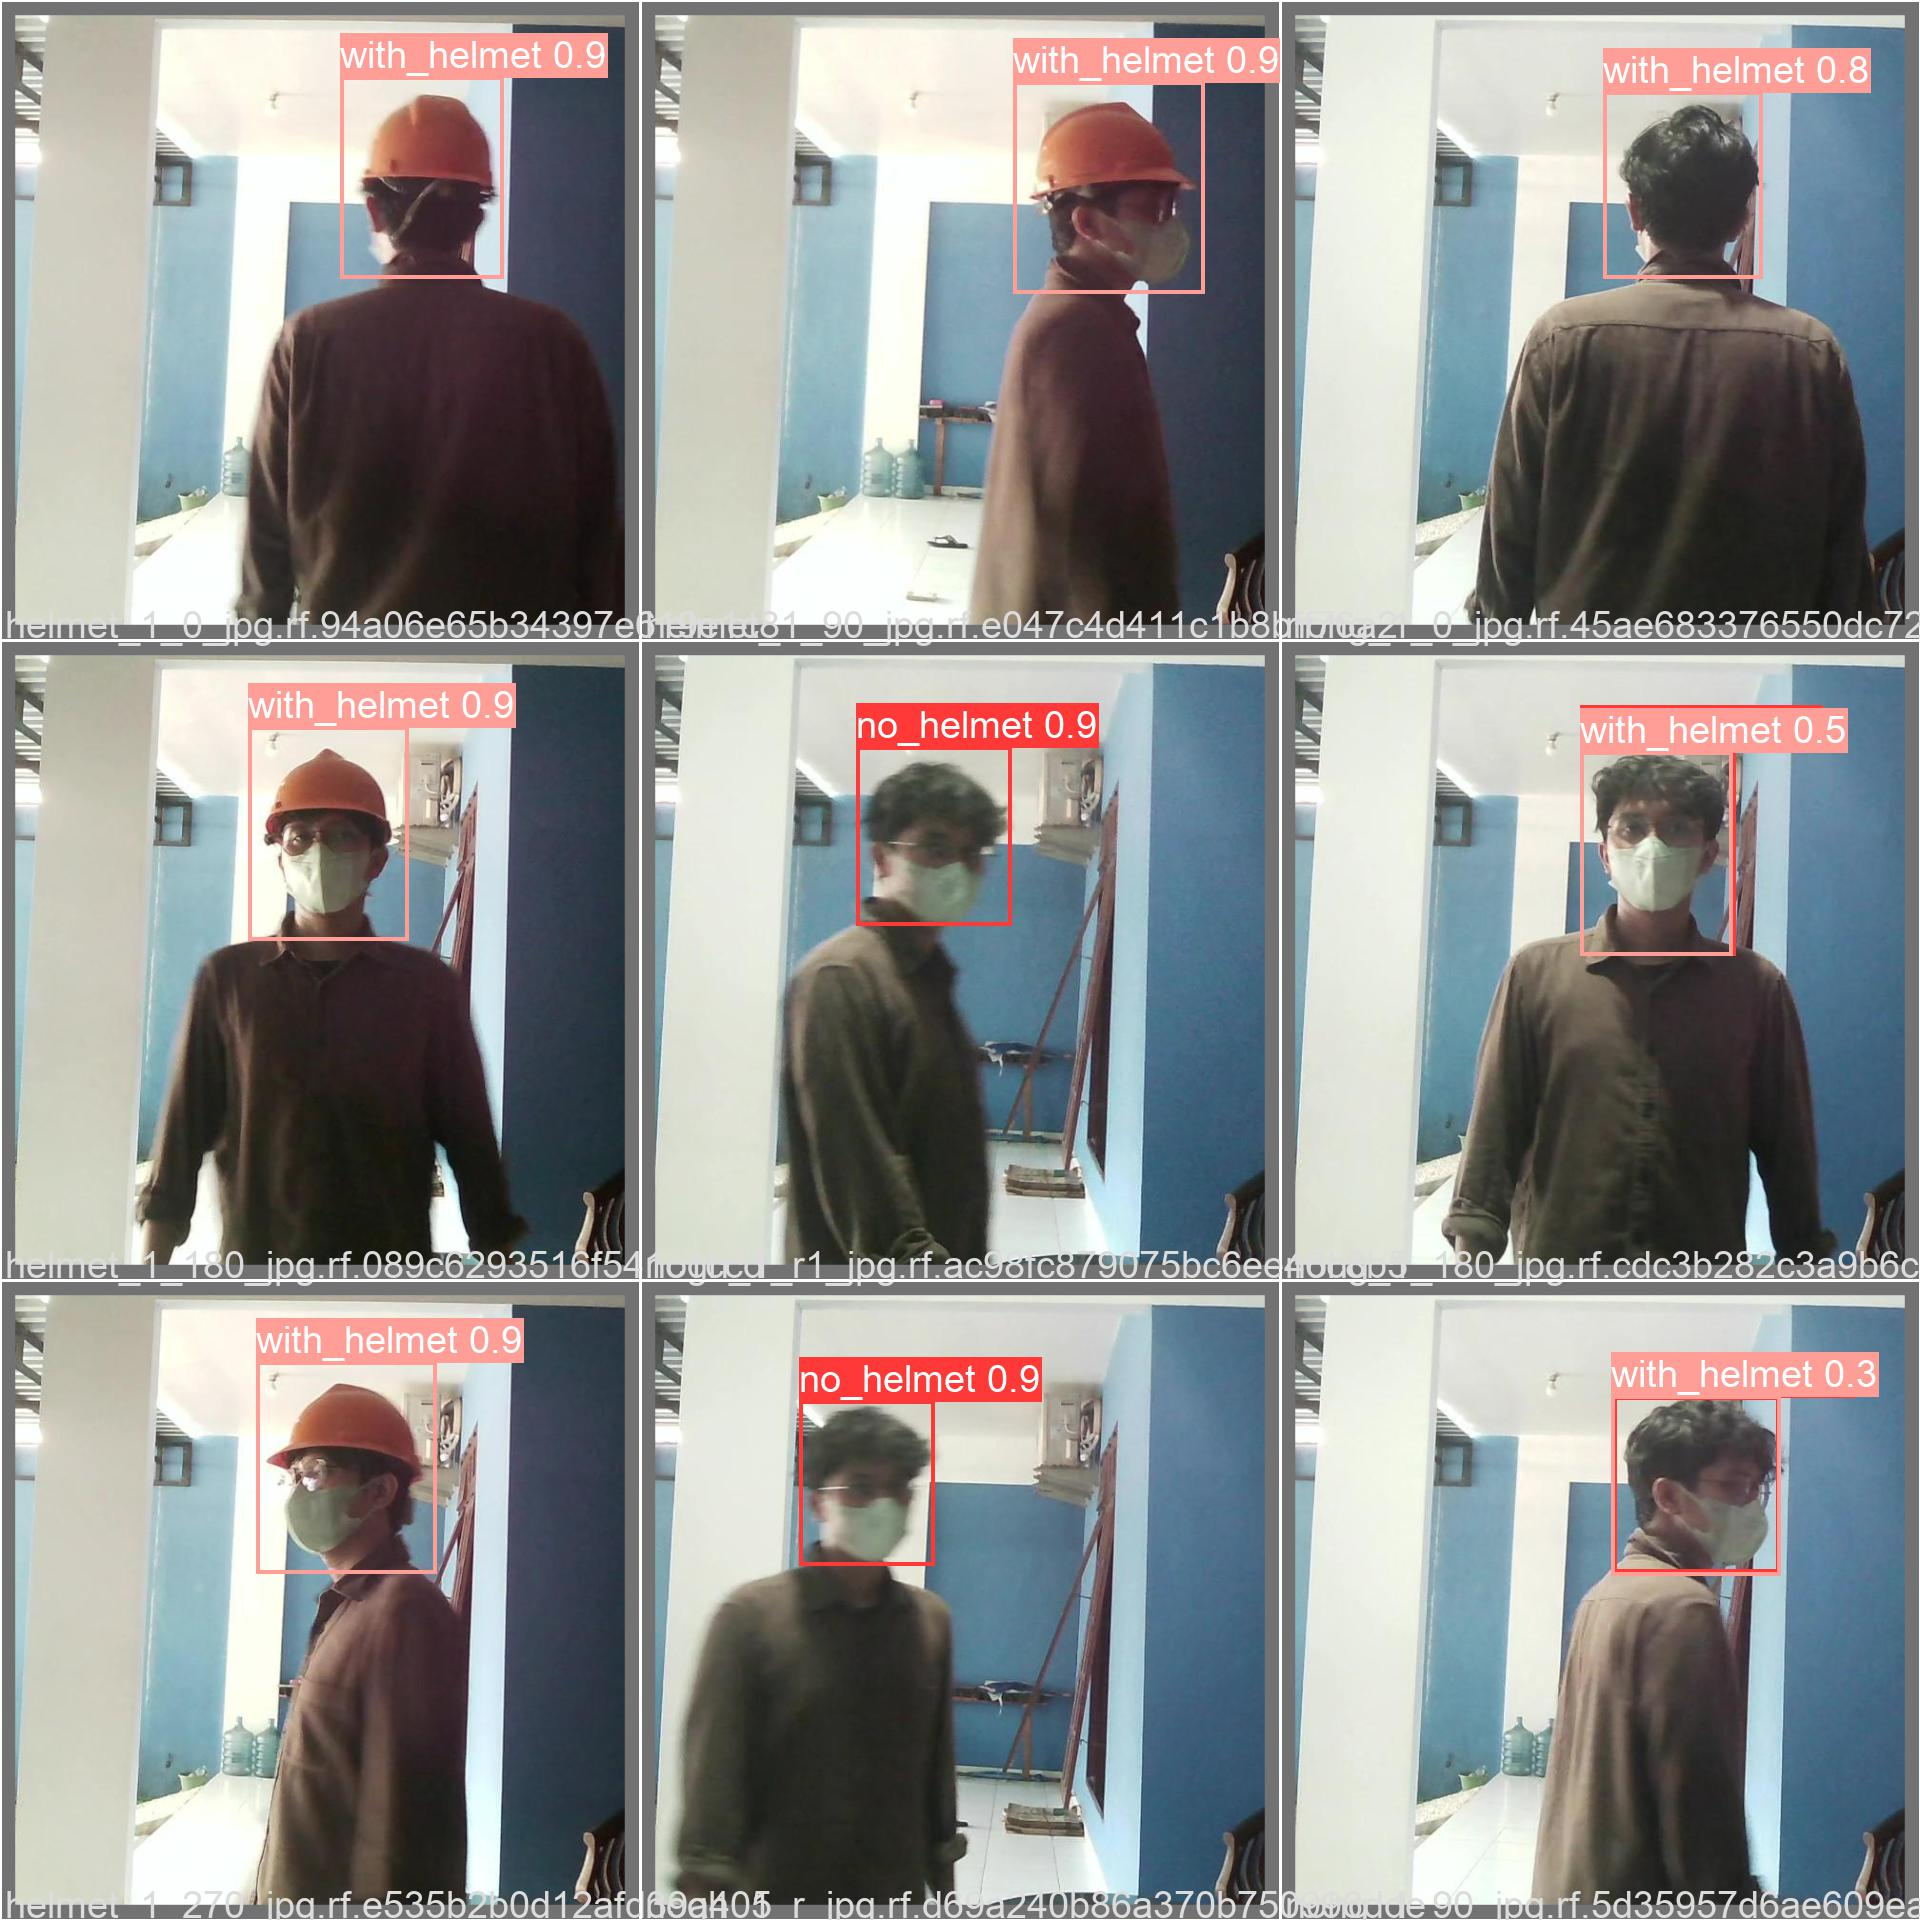
\includegraphics[scale=0.1]{gambar/BerdasarkanJarak/Jarak1_3/val_batch0_pred.jpg}
  \caption{Hasil Prediksi Pada Jarak 1.3 meter}
  % \label{fig:labelbaru}  
\end{figure}

\begin{longtable}{|c|c|c|c|}
  \caption{Konfigurasi Training menggunakan YOLOv5}
  \label{tb:wkwkw}\\
  \hline
  % \rowcolor[HTML]{C0C0C0}
  \textbf{\emph{Class} }                     & \textbf{\emph{Precision}}  & \textbf{\emph{Recall}} & \textbf{\emph{mAP@.5}}\\
  \hline
  all                                                 & 0.998           & 0.8     & 0.995         \\
  no\textunderscore helmet                            & 1               & 0.6       & 0.995          \\
  with\textunderscore helmet                          & 0.996           & 1       & 0.995            \\
  \hline
\end{longtable}

\subsection{Pengujian Pada Jarak 2.6 Meter}

\begin{figure}[ht]
  \centering
  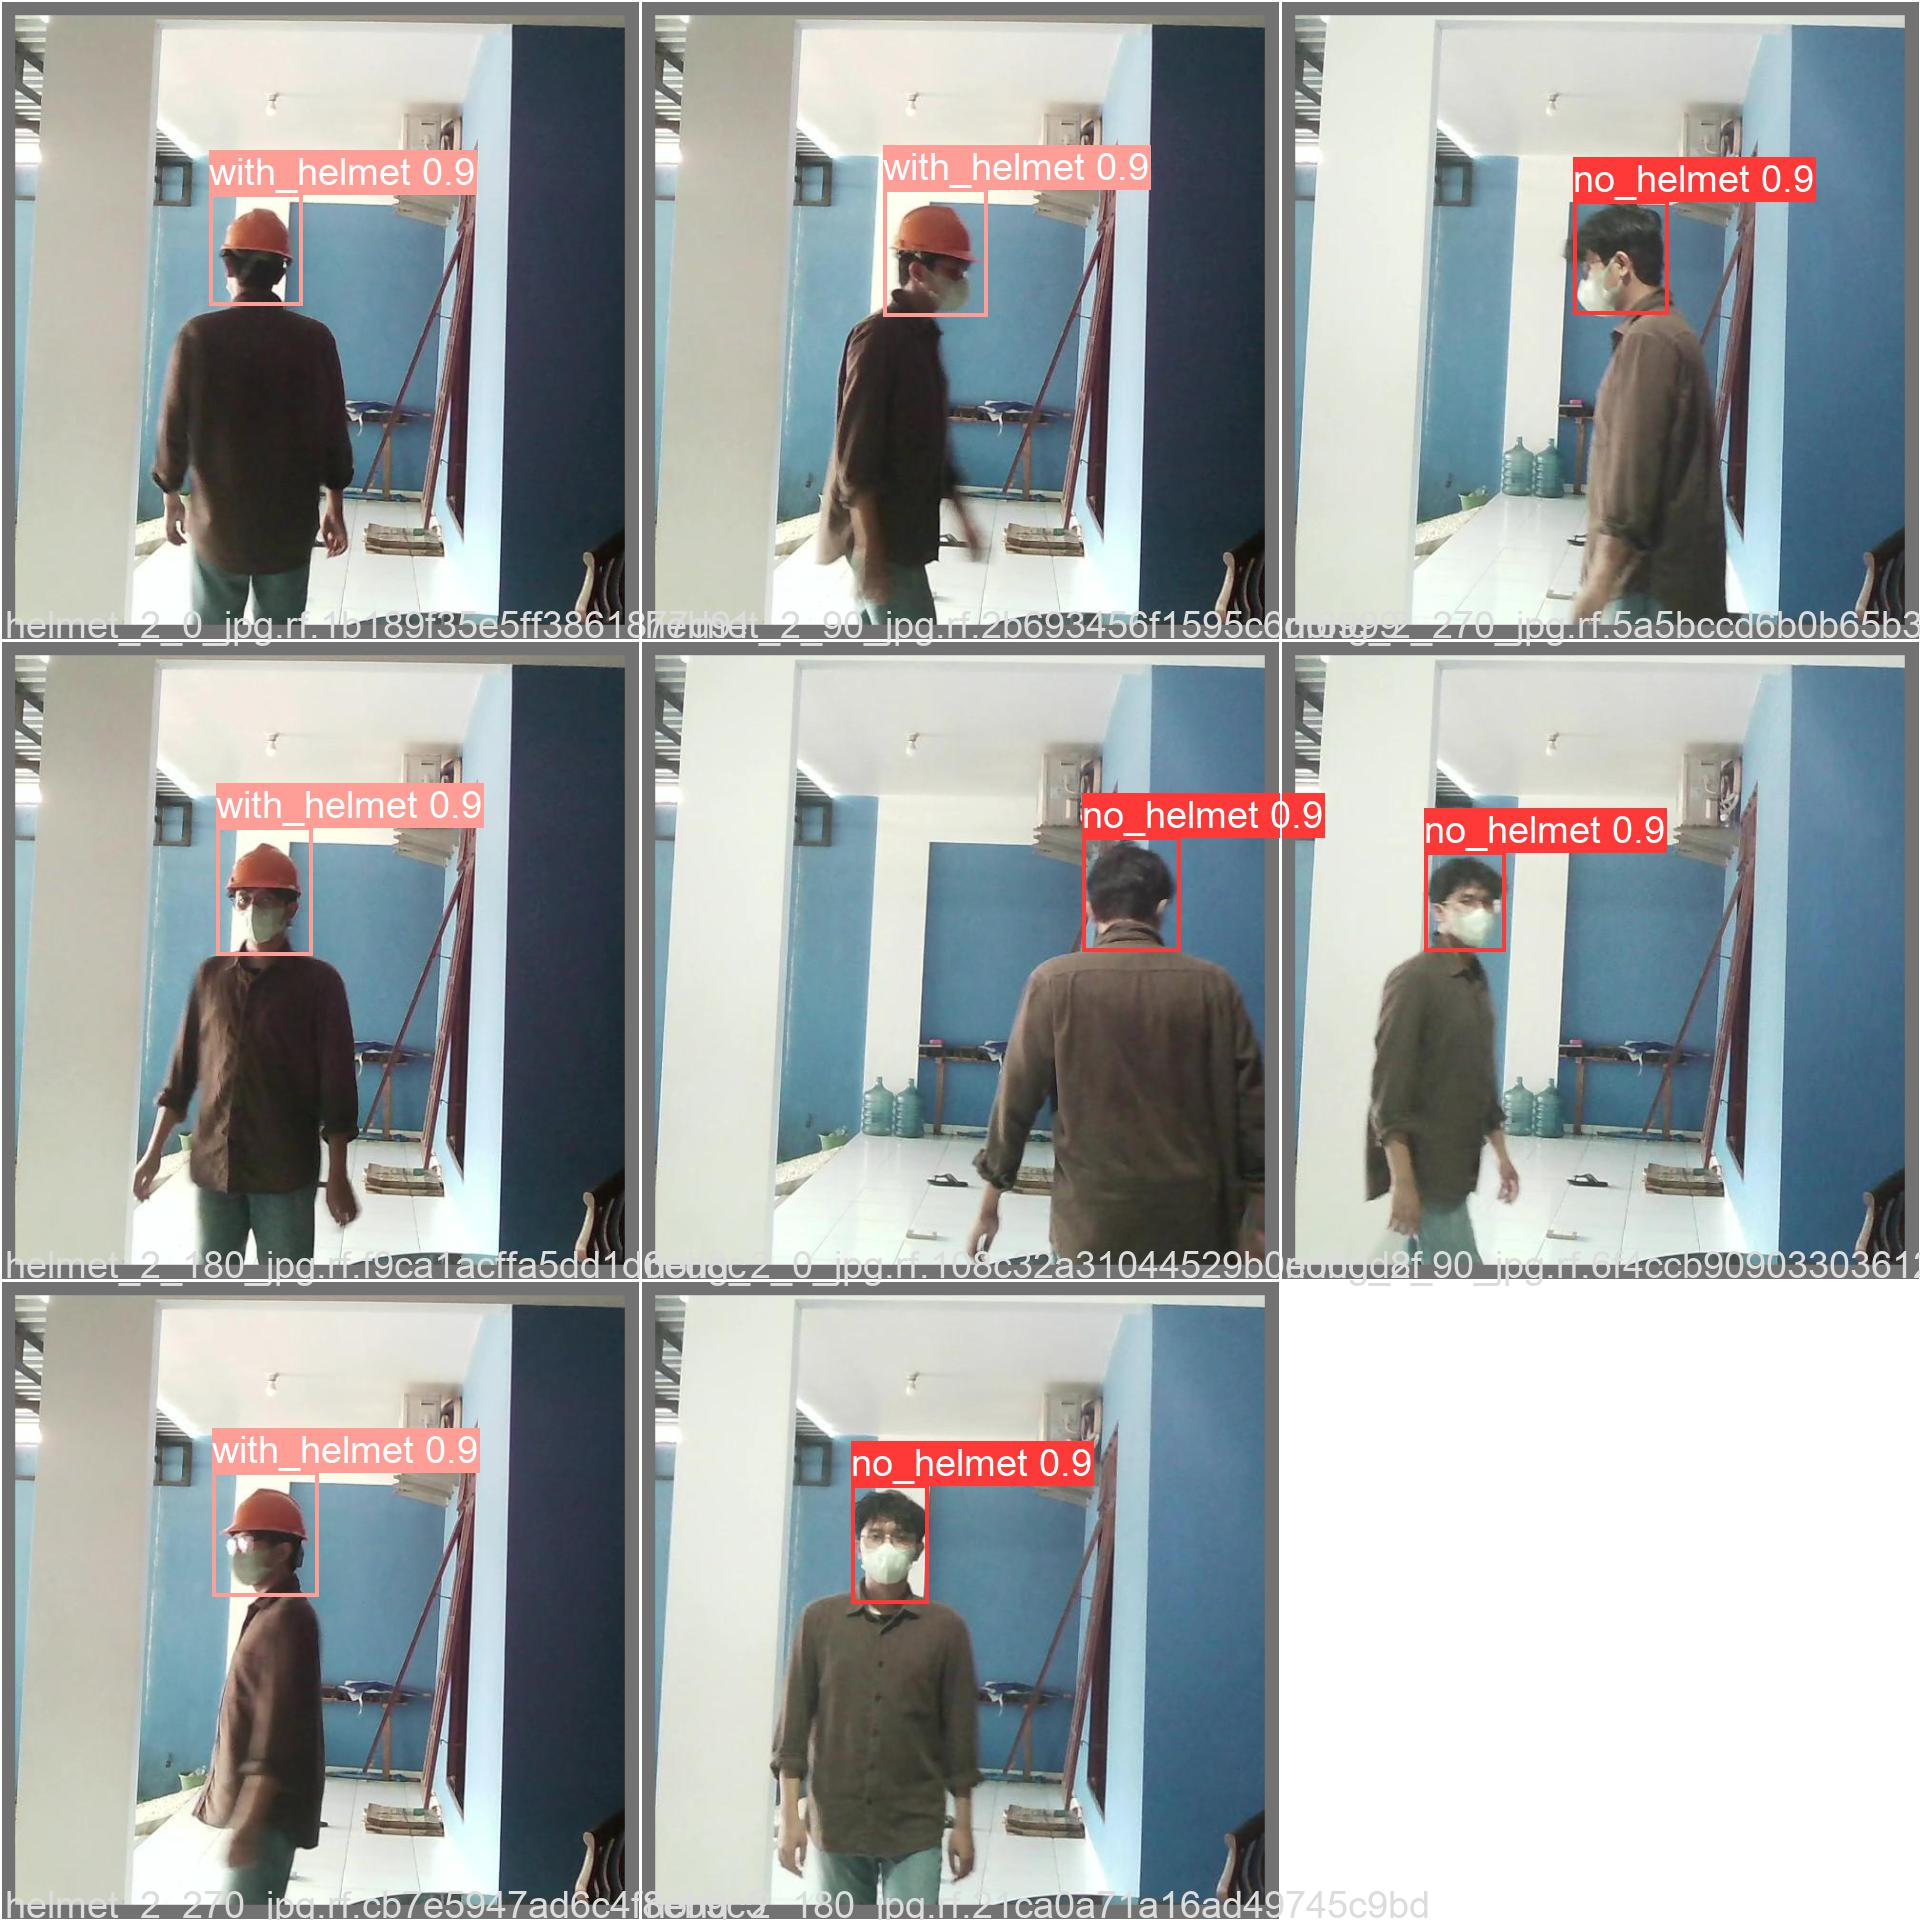
\includegraphics[scale=0.1]{gambar/BerdasarkanJarak/Jarak2_6/val_batch0_pred.jpg}
  \caption{Hasil Prediksi Pada Jarak 2.6 meter}
  % \label{fig:labelbaru}  
\end{figure}

\begin{longtable}{|c|c|c|c|}
  \caption{Konfigurasi Training menggunakan YOLOv5}
  \label{tb:jarak2_6}\\
  \hline
  % \rowcolor[HTML]{C0C0C0}
  \textbf{\emph{Class} }                     & \textbf{\emph{Precision}}  & \textbf{\emph{Recall}} & \textbf{\emph{mAP@.5}}\\
  \hline
  all                                                 & 0.996            & 1        & 0.995         \\
  no\textunderscore helmet                            & 1                & 1        & 0.995          \\
  with\textunderscore helmet                          & 0.992            & 1        & 0.995           \\
  \hline
\end{longtable}

\subsection{Pengujian Pada Jarak 4 Meter}

\begin{figure}[t]
  \centering
  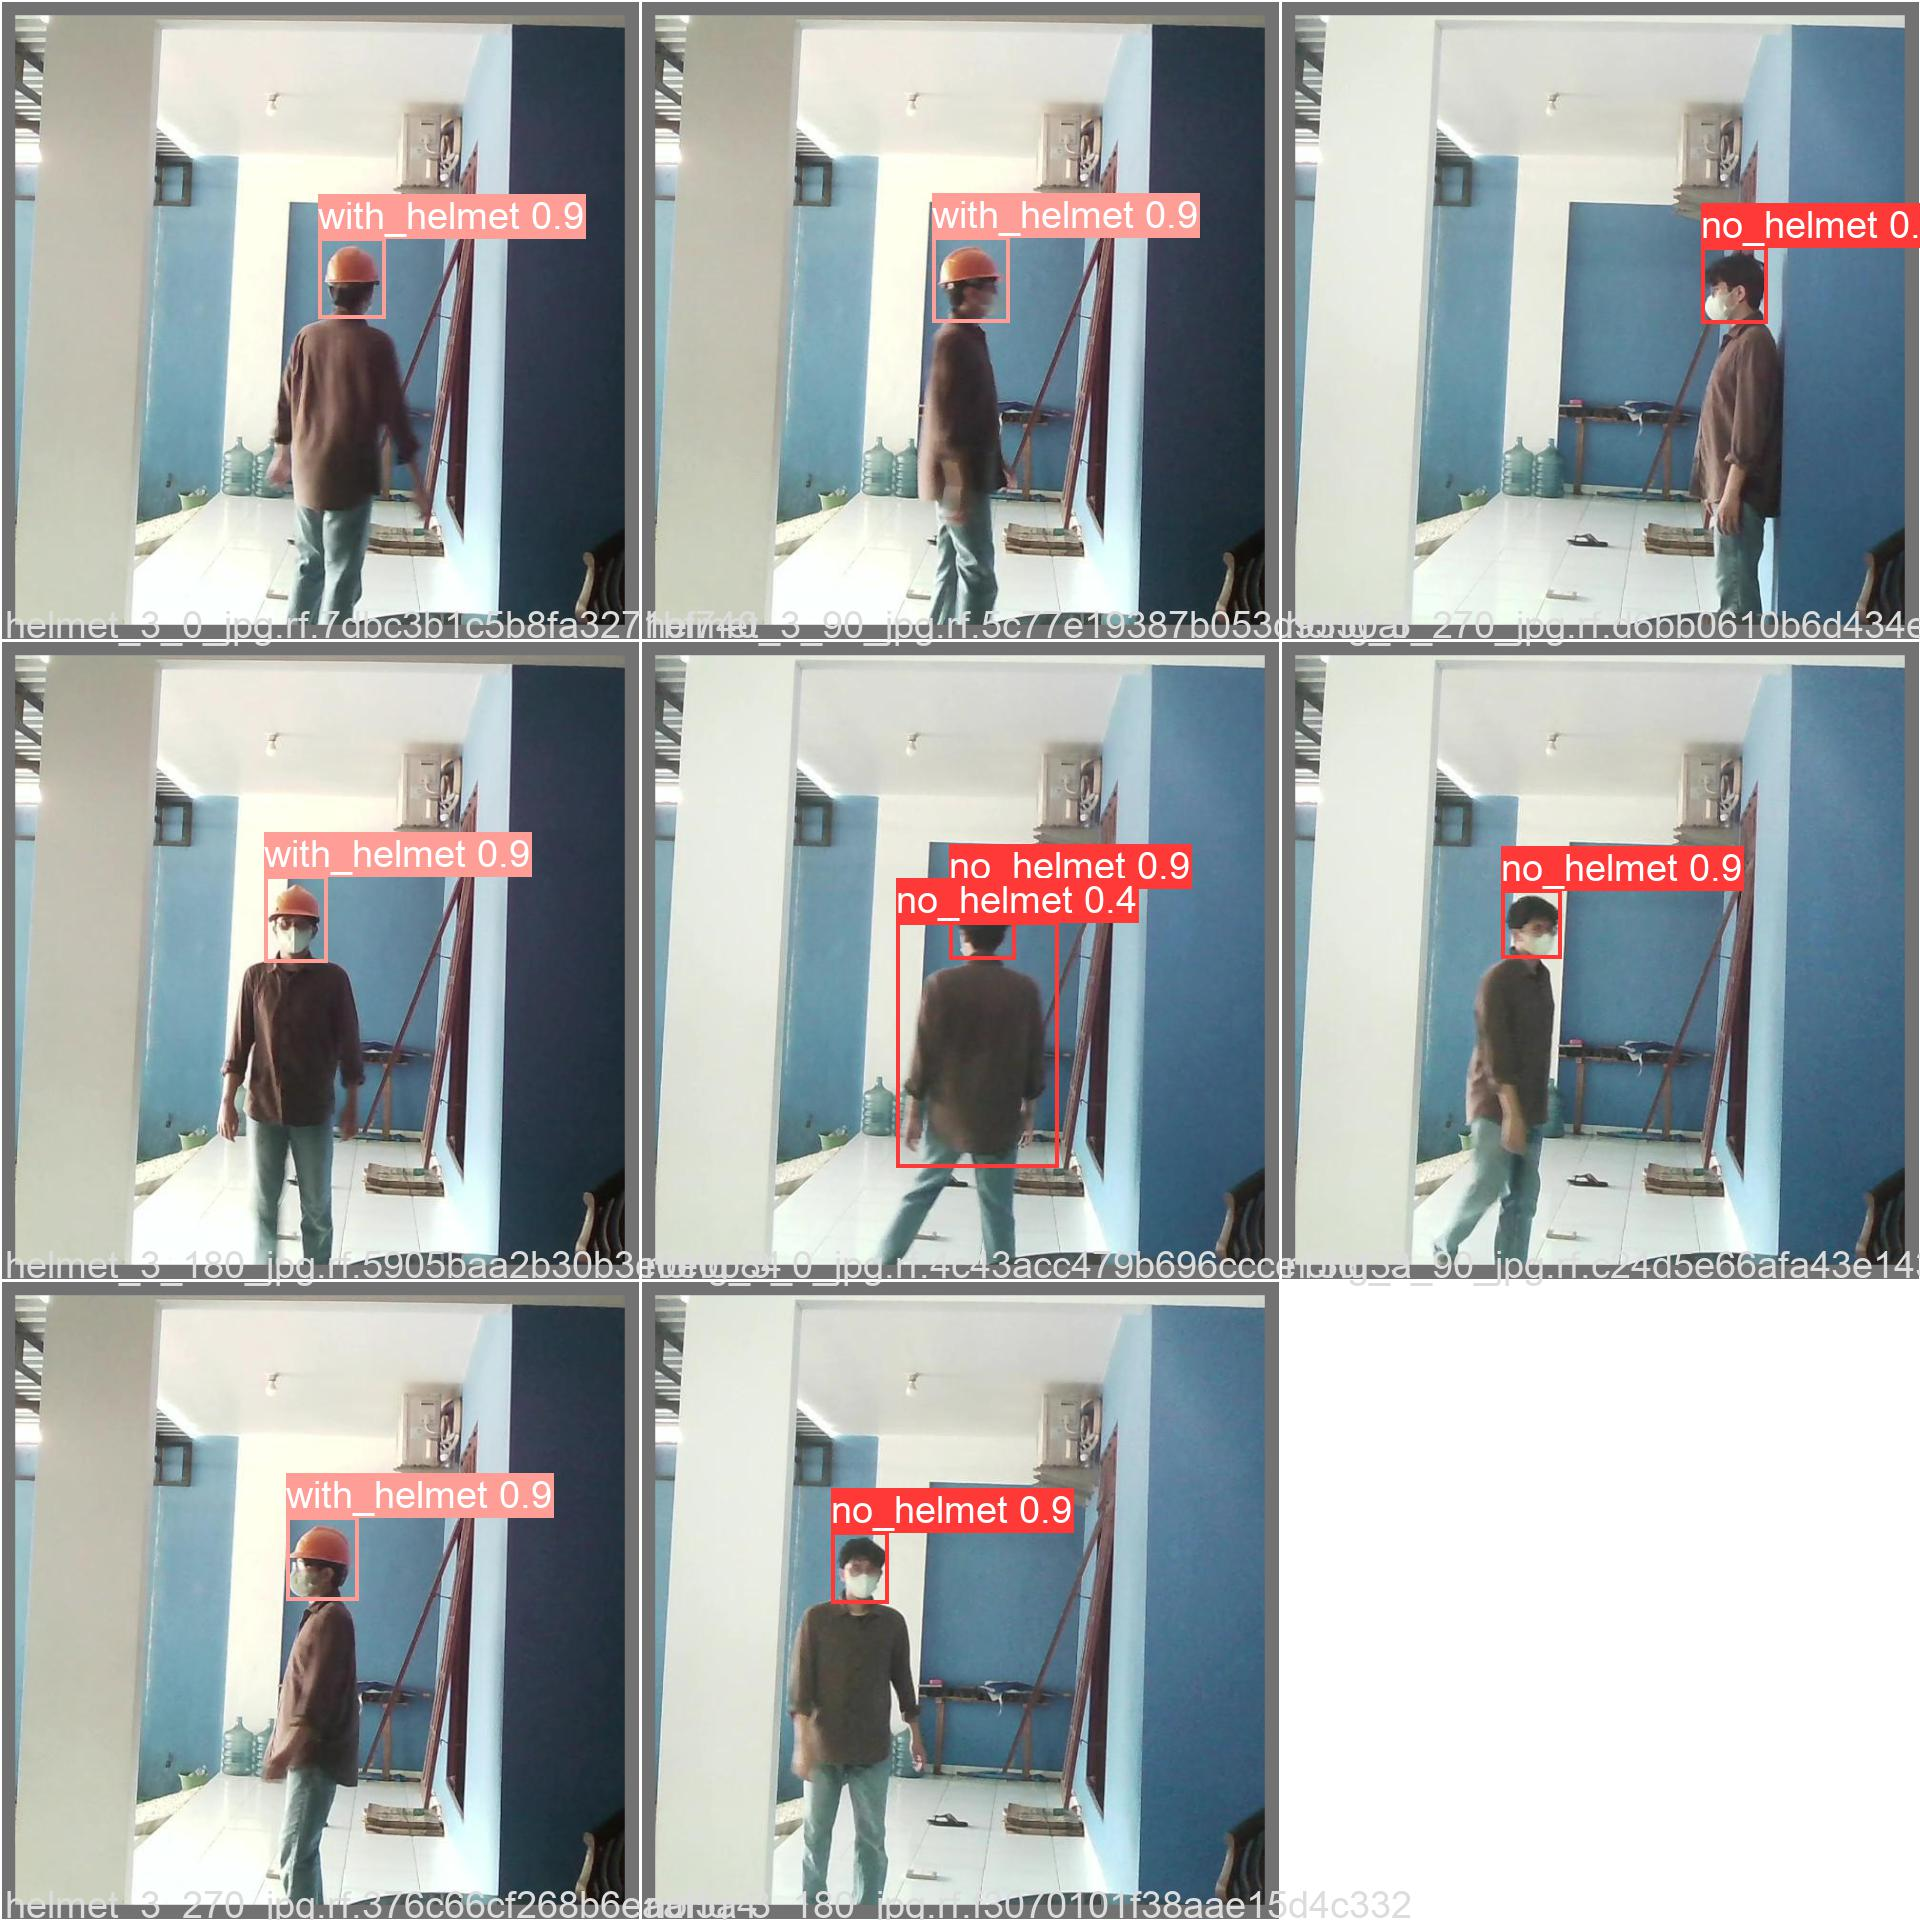
\includegraphics[scale=0.15]{gambar/BerdasarkanJarak/Jarak4/val_batch0_pred.jpg}
  \caption{Hasil Prediksi Pada Jarak 4 meter}
  % \label{fig:labelbaru}  
\end{figure}

\begin{longtable}{|c|c|c|c|}
  \caption{Konfigurasi Training menggunakan YOLOv5}
  \label{tb:jarak4}\\
  \hline
  % \rowcolor[HTML]{C0C0C0}
  \textbf{\emph{Class} }                     & \textbf{\emph{Precision}}  & \textbf{\emph{Recall}} & \textbf{\emph{mAP@.5}}\\
  \hline
  all                                                 & 0.981           & 1        & 0.995         \\
  no\textunderscore helmet                            & 1               & 1        & 0.995          \\
  with\textunderscore helmet                          & 0.963           & 1        & 0.995           \\
  \hline
\end{longtable}

\subsection{Pengujian Pada Jarak 5.3 Meter}

Hasil validasi untuk jarak 5.3 meter masih memiliki tingkat presisi diatas 0.9.

\begin{figure}[ht]
  \centering
  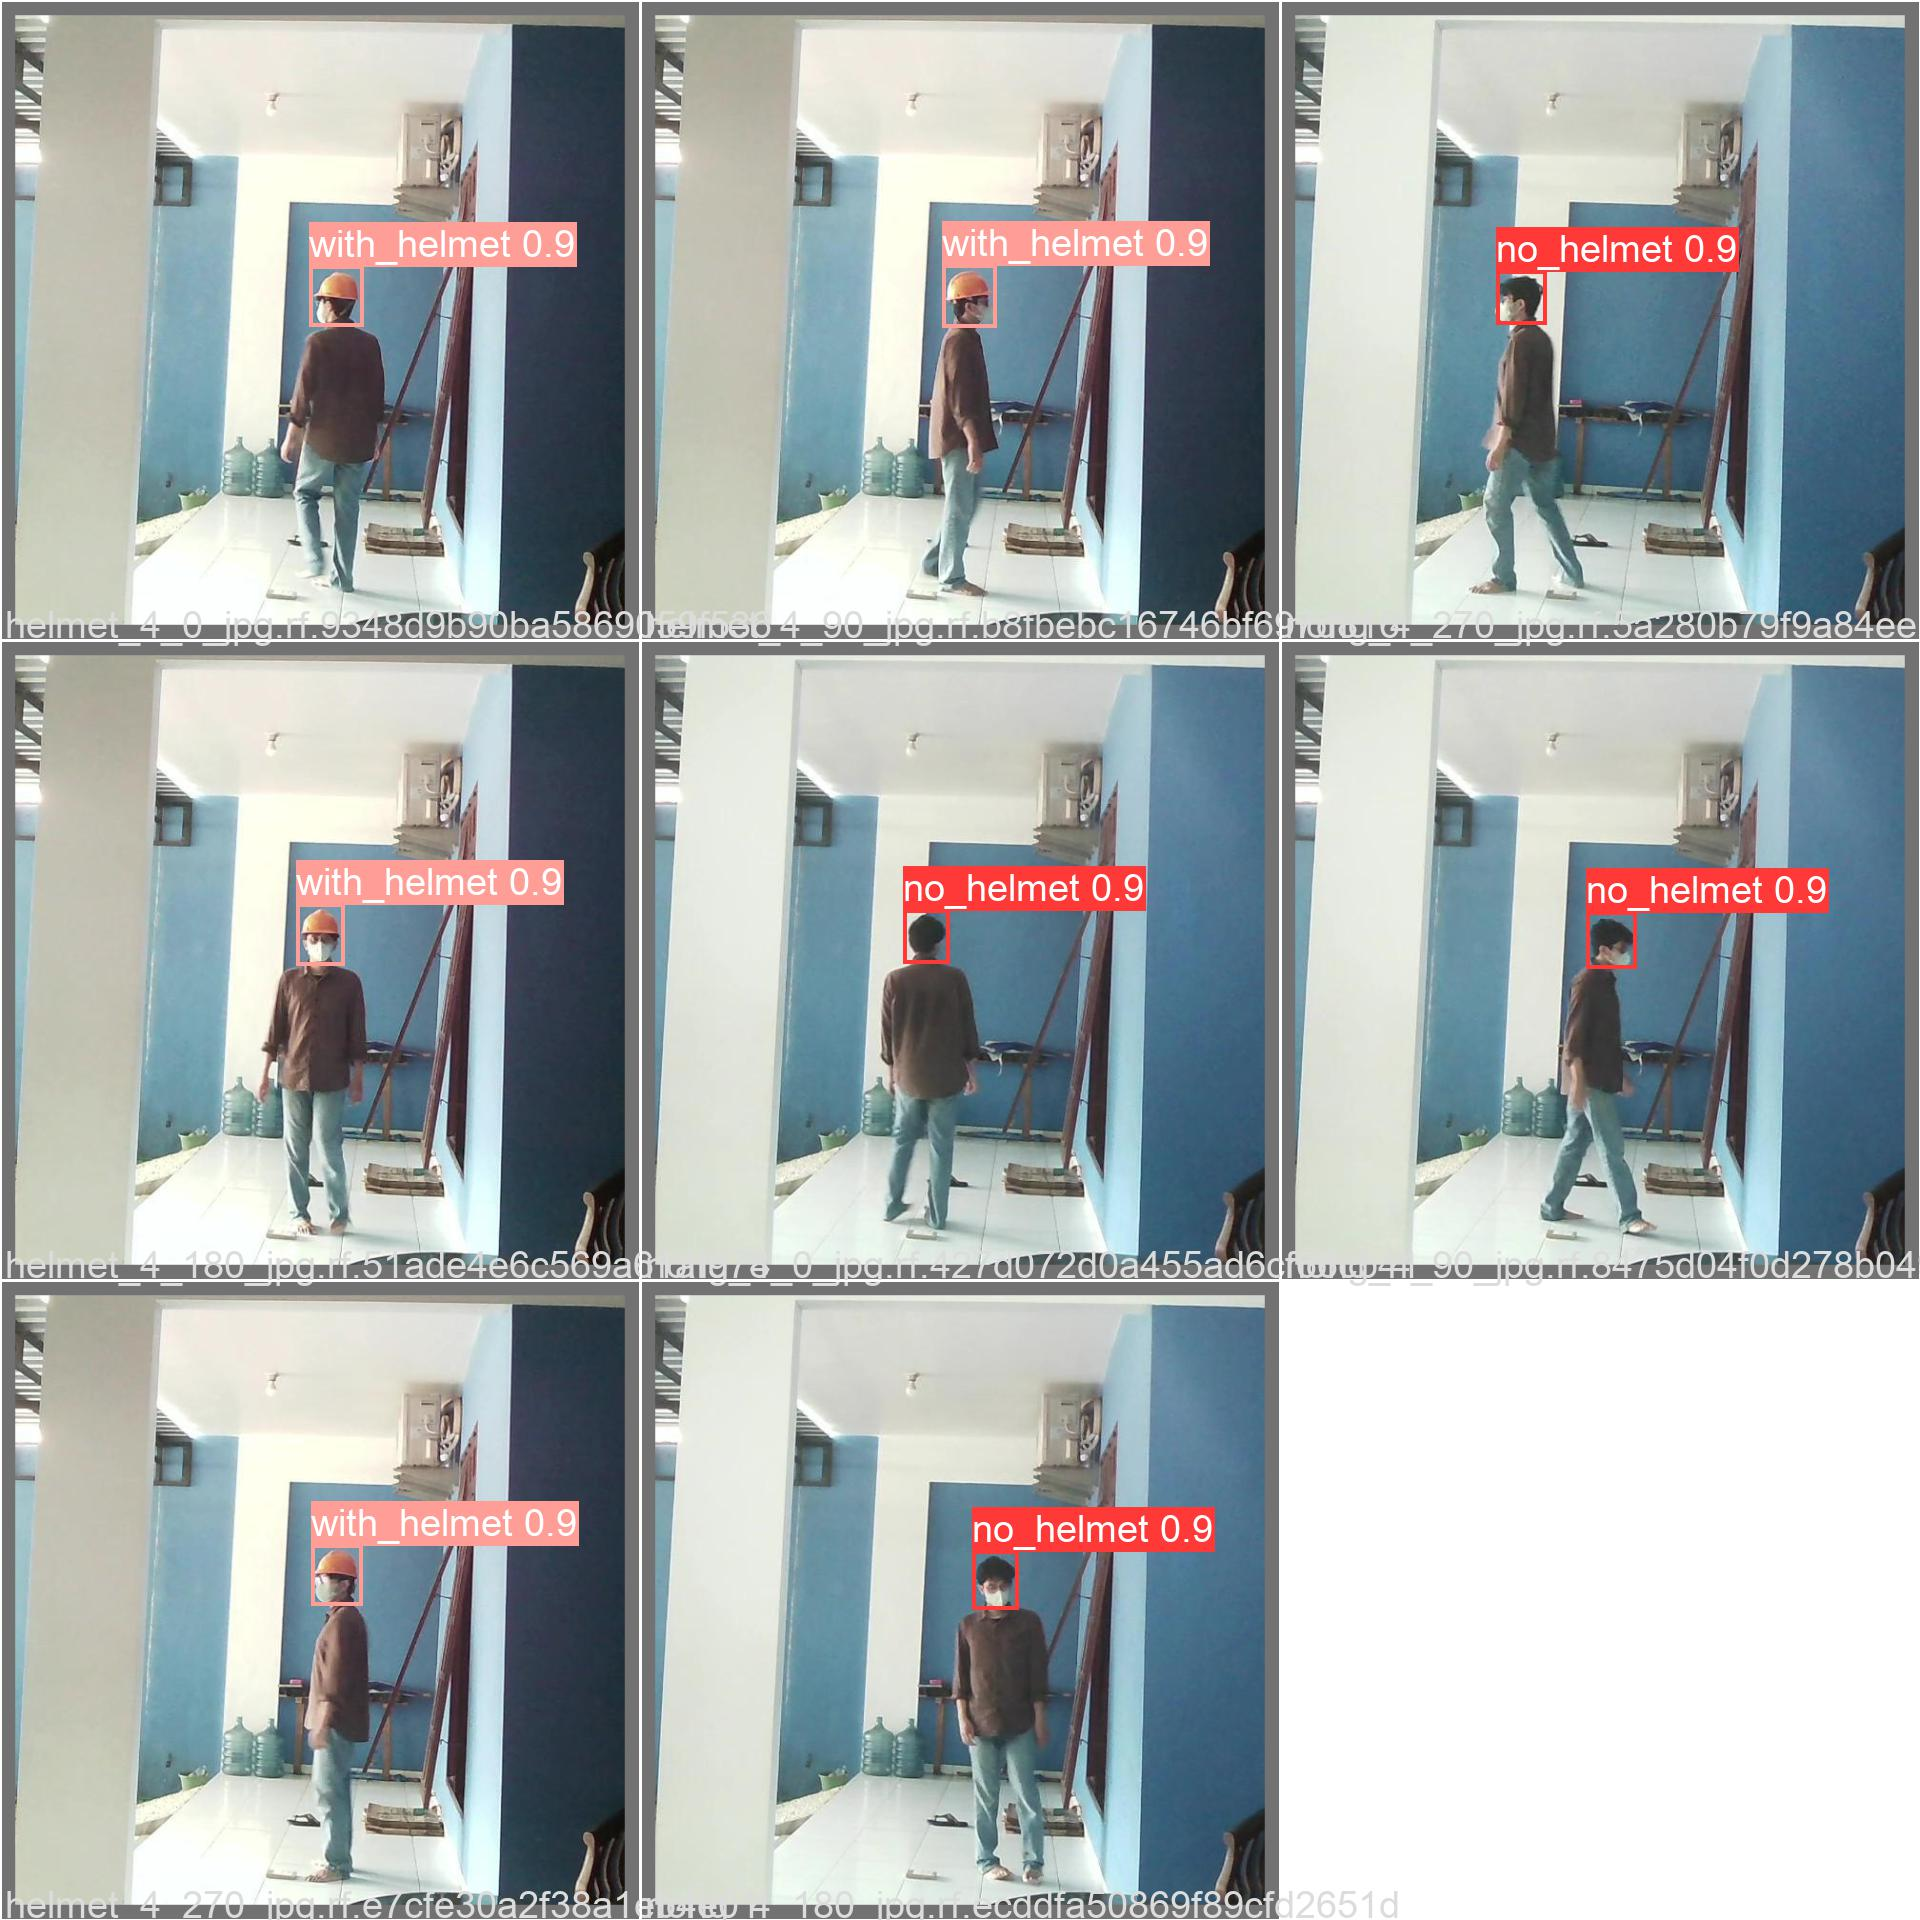
\includegraphics[scale=0.15]{gambar/BerdasarkanJarak/Jarak5_3/val_batch0_pred.jpg}
  \caption{Hasil Prediksi Pada Jarak 5.3 meter}
  % \label{fig:labelbaru}  
\end{figure}

\begin{longtable}{|c|c|c|c|}
  \caption{Konfigurasi Training menggunakan YOLOv5}
  \label{tb:jarak5_3}\\
  \hline
  % \rowcolor[HTML]{C0C0C0}
  \textbf{\emph{Class} }                     & \textbf{\emph{Precision}}  & \textbf{\emph{Recall}} & \textbf{\emph{mAP@.5}}\\
  \hline
  all                                                 & 0.997           & 1        & 0.995         \\
  no\textunderscore helmet                            & 1               & 1        & 0.995          \\
  with\textunderscore helmet                          & 0.995           & 1        & 0.995           \\
  \hline
\end{longtable}

\subsection{Pengujian Pada Jarak 6.7 Meter}

\begin{figure}[H]
  \centering
  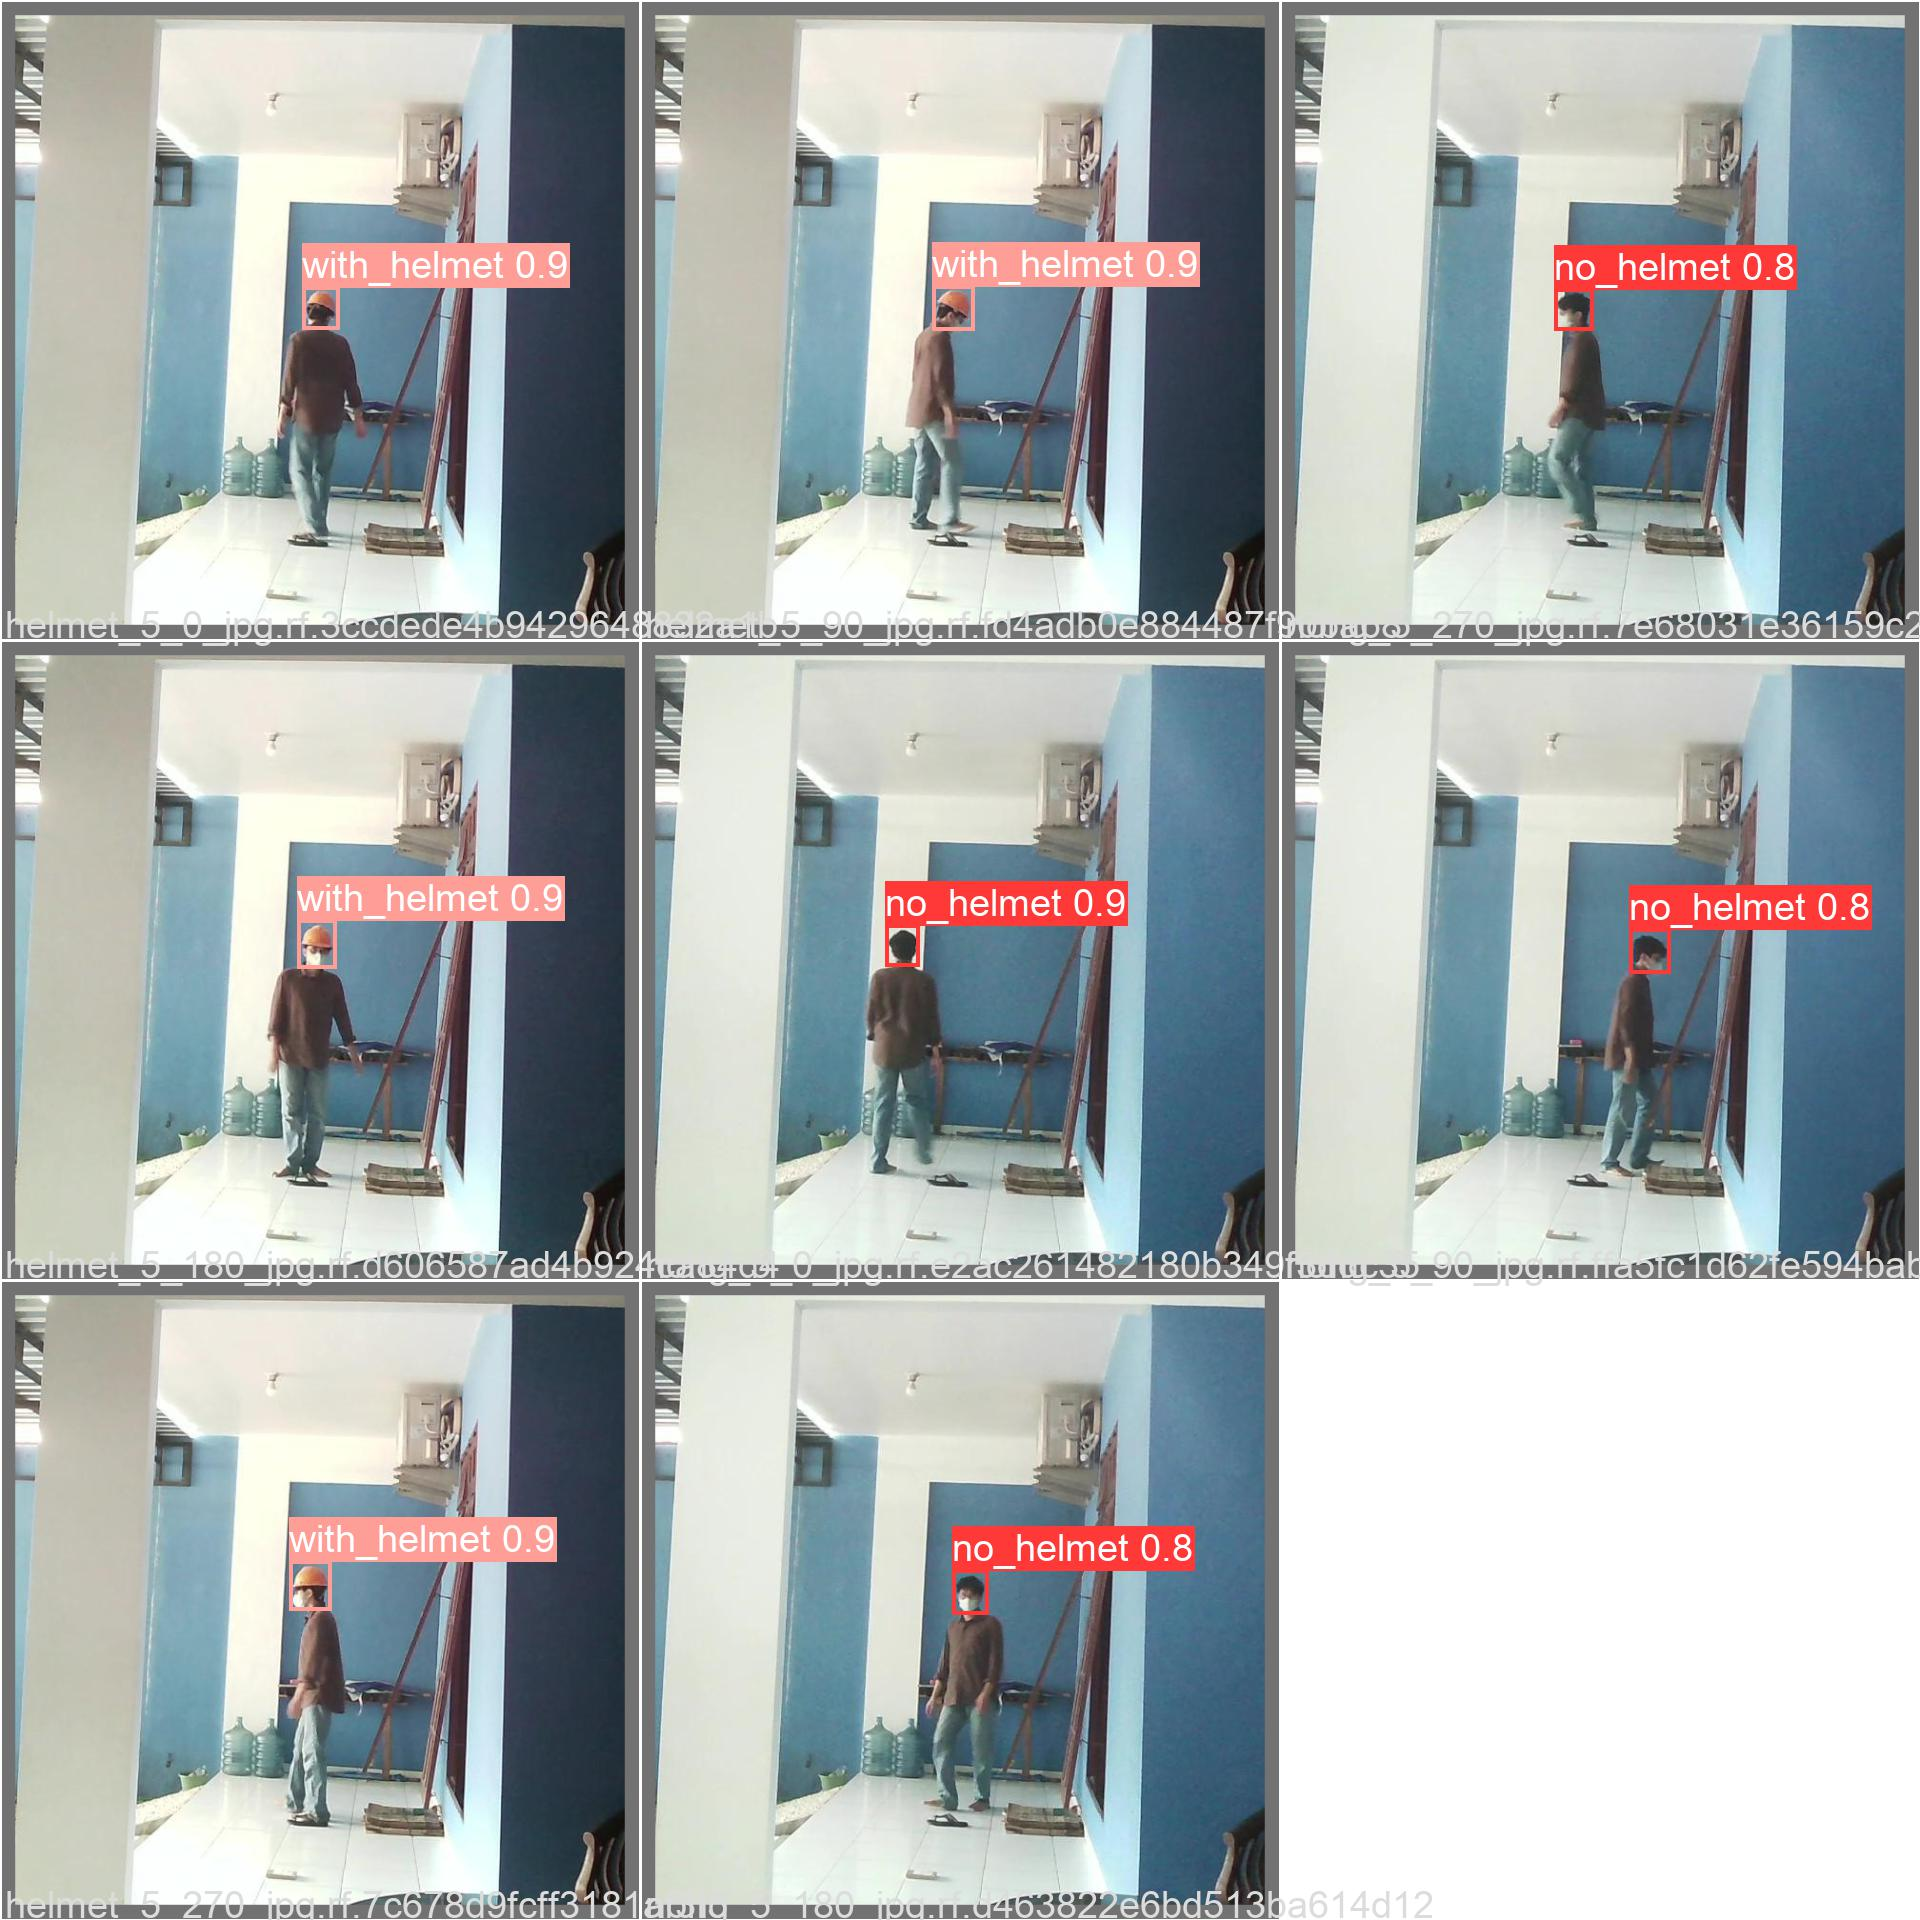
\includegraphics[scale=0.1]{gambar/BerdasarkanJarak/Jarak6_7/val_batch0_pred.jpg}
  \caption{Hasil Prediksi Pada Jarak 6.7 meter}
  % \label{fig:labelbaru}  
\end{figure}

\begin{longtable}{|c|c|c|c|}
  \caption{Konfigurasi Training menggunakan YOLOv5}
  \label{tb:jarak6_7}\\
  \hline
  % \rowcolor[HTML]{C0C0C0}
  \textbf{\emph{Class} }                     & \textbf{\emph{Precision}}  & \textbf{\emph{Recall}} & \textbf{\emph{mAP@.5}}\\
  \hline
  all                                                 & 0.993           & 1        & 0.995         \\
  no\textunderscore helmet                            & 1               & 1        & 0.995          \\
  with\textunderscore helmet                          & 0.986           & 1        & 0.995           \\
  \hline
\end{longtable}


\subsection{Pengujian Pada Jarak 9 Meter}
\label{}

\begin{figure}[ht]
  \centering
  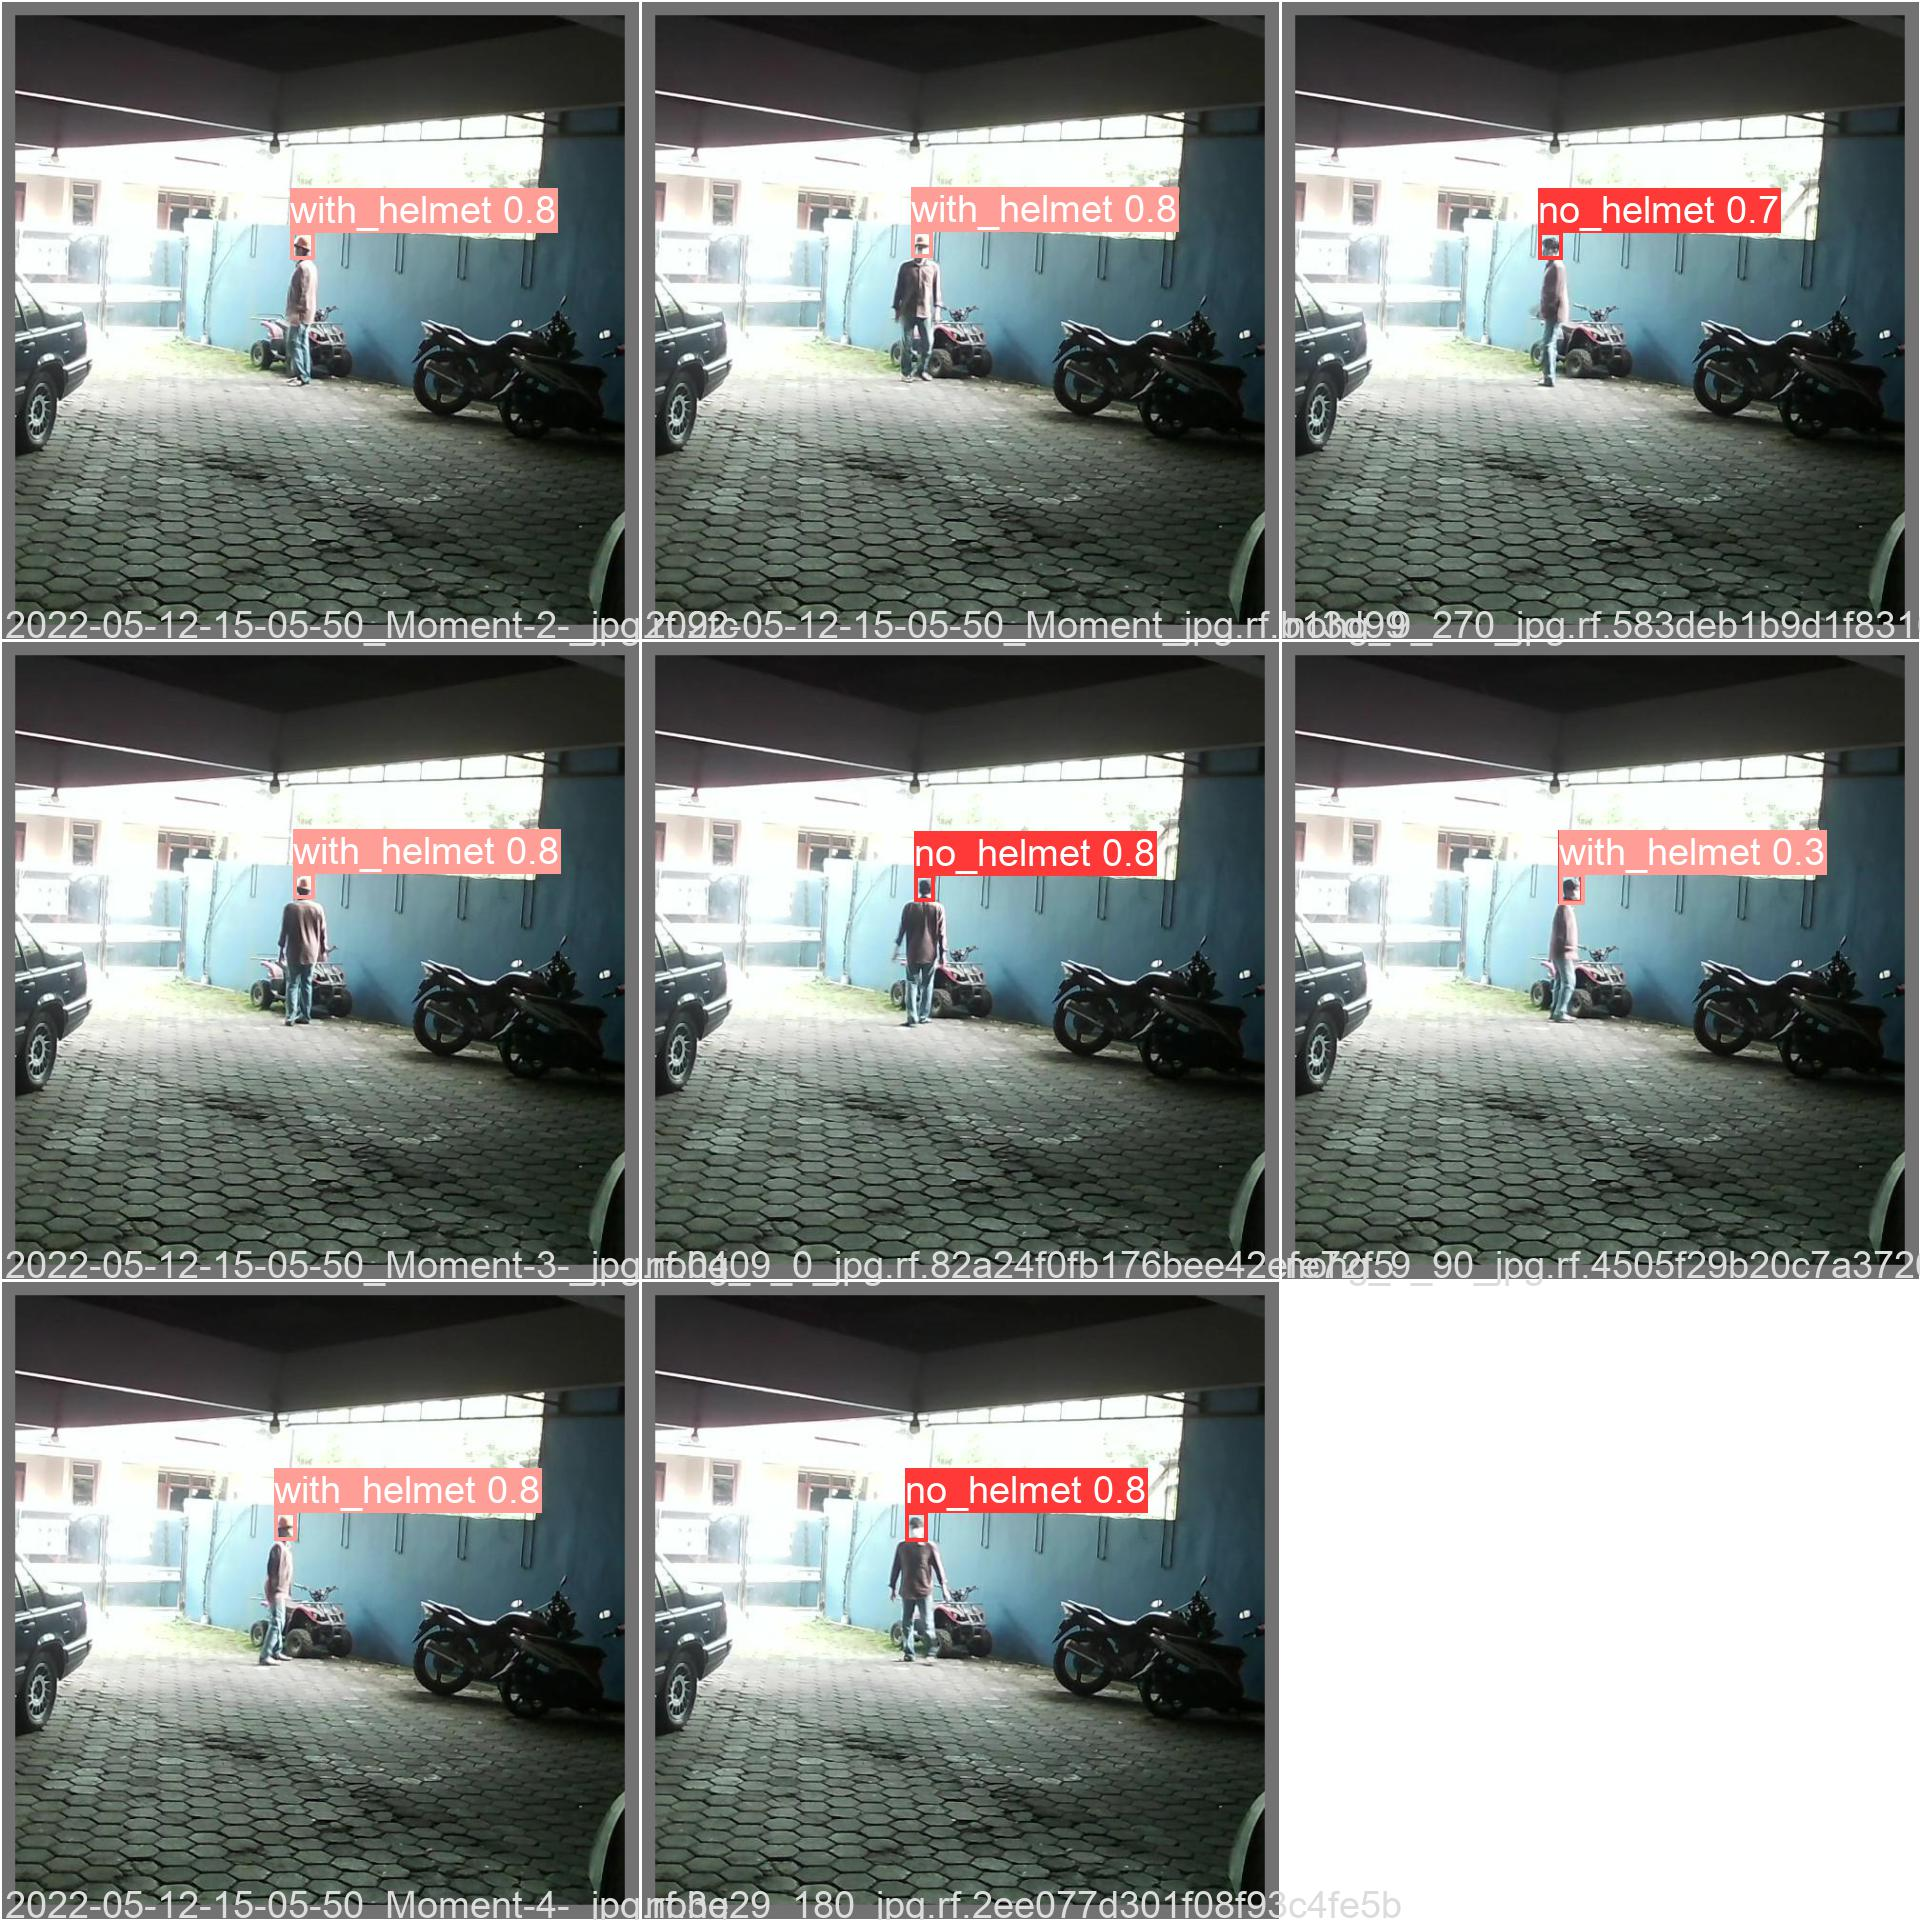
\includegraphics[scale=0.1]{gambar/BerdasarkanJarak/Jarak9/val_batch0_pred.jpg}
  \caption{Hasil Prediksi Pada Jarak 9 meter}
  % \label{fig:labelbaru}  
\end{figure}

\begin{longtable}{|c|c|c|c|}
  \caption{Konfigurasi Training menggunakan YOLOv5}
  \label{tb:jarak9}\\
  \hline
  % \rowcolor[HTML]{C0C0C0}
  \textbf{\emph{Class} }                     & \textbf{\emph{Precision}}  & \textbf{\emph{Recall}} & \textbf{\emph{mAP@.5}}\\
  \hline
  all                                                 & 0.959          & 1        & 0.995         \\
  no\textunderscore helmet                            & 1               & 1        & 0.995          \\
  with\textunderscore helmet                          & 0.918           & 1        & 0.995           \\
  \hline
\end{longtable}

\section{Pengujian Pada Tingkat Kecerahan Rendah}
\label{sec:pengujianberdasarkantingkatkeceharan}

\par Bagian ini memaparkan performa model melakukan
deteksi pada input gambar dengan tingkat kecerahan rendah. Data validasi berisi
35 gambar dengan jumlah label \emph{no\textunderscore helmet} 20 dan label \emph{with\textunderscore helmet} 57.
Validasi dilakukan pada bobot hasil training yang menggunakan \textit{pretrained weight} dan yang tanpa menggunakan \textit{pretrained weight}. 

\subsection{Pengujian Pada Tingkat Kecerahan Rendah dengan \emph{Pretrained Weight}}
\label{subsec:lowlight_pretrained}

\par Berikut meruoakan pemaparan hasil validasi pada data validasi menggunakan \emph{weight} yang di-\emph{train} menggunakan
\emph{pretrained weights} yang disedikan repo YOLOv5. Seperti yang dijelaskan pada Subbab~\ref{subsec:ujiperforma_coco}. 

\subsubsection{\emph{Pretrained}  YOLOv5n}
\label{subsubsec:lowlight_yolov5n}

\par Dilakukan pengujian kecerahan rendah dengan menggunakan bobot yang di-\emph{train} menggunakan bobot
pretrain COCO untuk varian \emph{nano} yang merupakan varian paling kecil dari semua bobot yang disediakan 
dari repo. Didapatkan rata - rata presisi untuk semua kelas 0.767 dan \emph{recall} untuk semua kelas 0.373.
\par Didapati untuk kelas \emph{no\textunderscore helmet} mendapatkan nilai \emph{precision} 1 dan \emph{recall}
0. Hal ini dikarenakan objek kepala tanpa menggunakan helm tidak ada yang terdektsi dan atau terdeteksi
sebagai kelas \emph{with\textunderscore helmet}. 

\begin{longtable}{|c|c|c|c|}
  \caption{Hasil Validasi Pada Tingkat Kecerahan Rendah dengan \emph{Pretrained YOLOv5n}}
  \label{tb:validasitingkatacerahrendah_yolo5n}\\
  \hline
  % \rowcolor[HTML]{C0C0C0}
  \textbf{\emph{Class} }                     & \textbf{\emph{Precision}}  & \textbf{\emph{Recall}} & \textbf{\emph{mAP@.5}}\\
  \hline
  all                                                 & 0.767          & 0.373        & 0.415         \\
  no\textunderscore helmet                            & 1              & 0            & 0.143          \\
  with\textunderscore helmet                          & 0.534          & 0.745        & 0.687         \\
  \hline
\end{longtable}

\begin{figure}[ht]
  \centering
  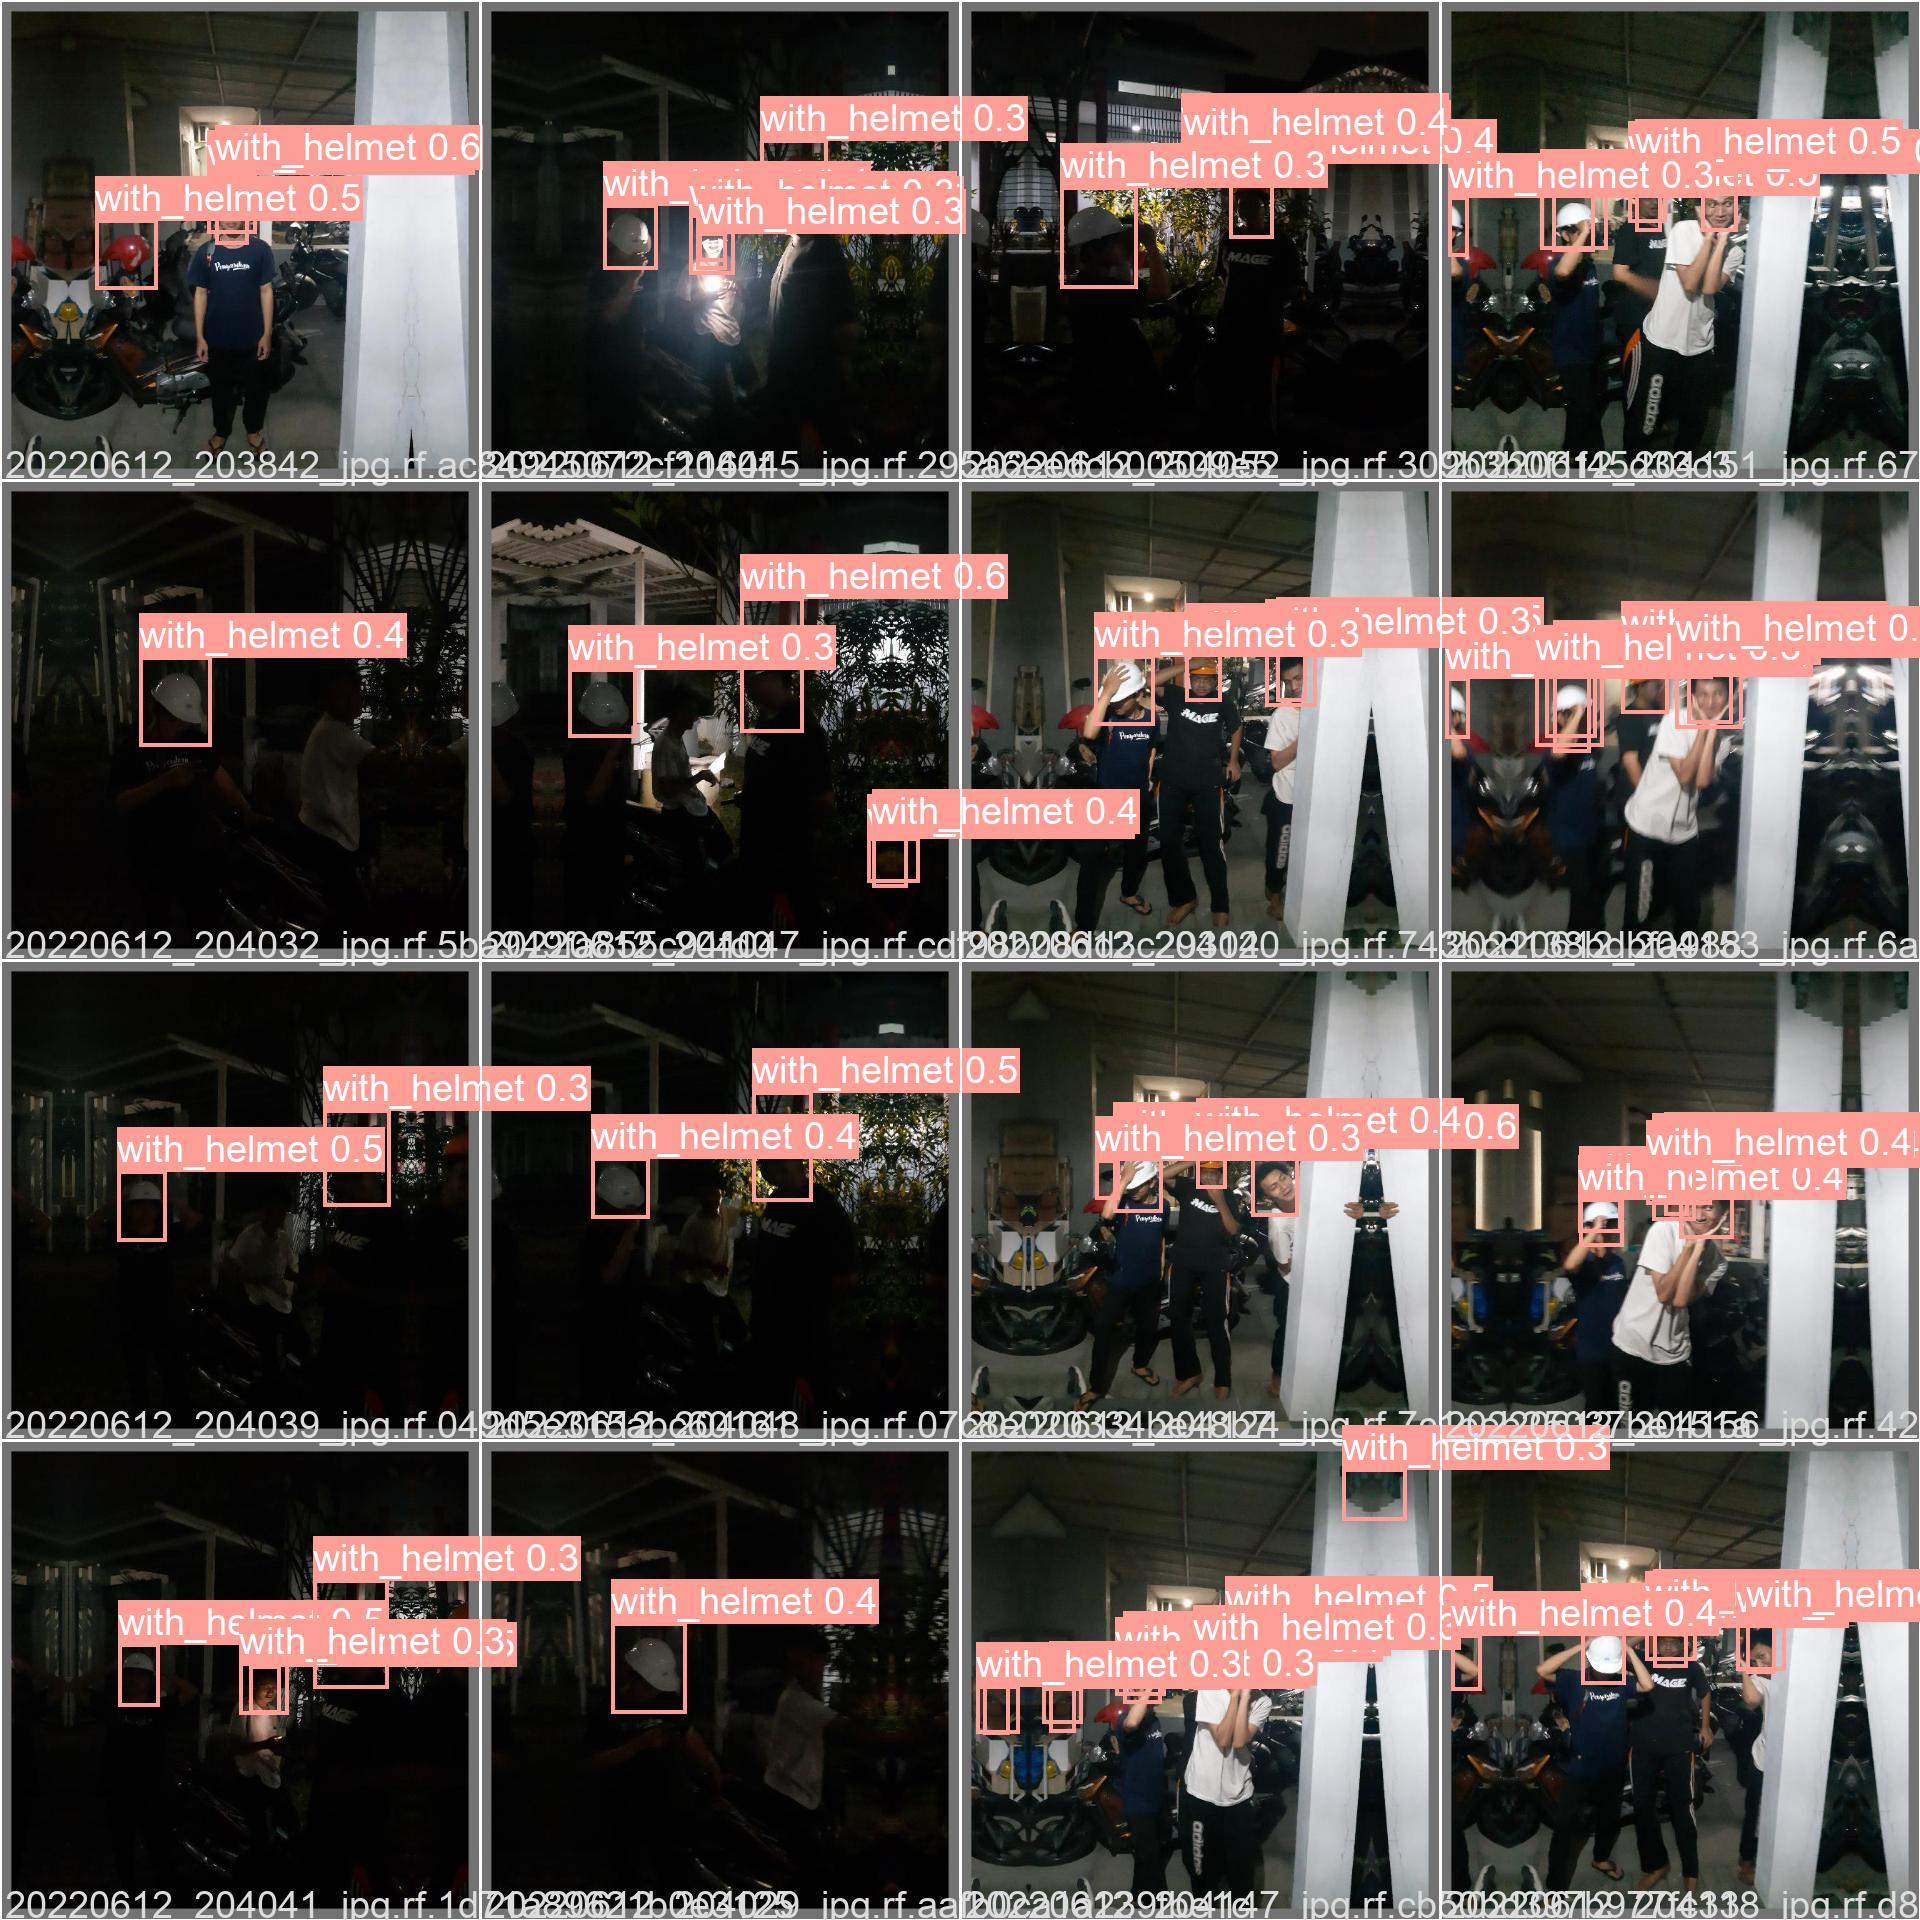
\includegraphics[scale=0.1]{gambar/train_v2_val/low_ligjt/yolonano/val_batch0_pred.jpg}
  \includegraphics[scale=0.1]{gambar/train_v2_val/low_ligjt/yolonano/val_batch0_labels.jpg}
  \caption{Hasil Prediksi dengan Validation Set Pada Keadaan Rendah dengan Pretrain YOLOv5n}
  % \label{fig:labelbaru}  
\end{figure}

\subsubsection{\emph{Pretrained} YOLOv5s}
\label{subsubsec:lowlight_yolov5s}

\par Dilakukan pengujian kecerahan rendah dengan menggunakan bobot yang di-\emph{train} menggunakan bobot
pretrain COCO untuk varian \emph{small}. Didapatkan rata - rata presisi untuk semua kelas 0.775 dan \emph{recall} untuk semua
kelas 0.799. Terdapat beberapa \emph{False Positive} dalam prediksi yaitu helm motor yang diletakkan diatas
motor diprediksi sebagai \emph{with\textunderscore helmet} begitu juga.

\begin{longtable}{|c|c|c|c|}
  \caption{Hasil Validasi Pada Tingkat Kecerahan Rendah dengan \emph{Pretrained YOLOv5s}}
  \label{tb:validasitingkatacerahrendah_yolov5s}\\
  \hline
  % \rowcolor[HTML]{C0C0C0}
  \textbf{\emph{Class} }                     & \textbf{\emph{Precision}}  & \textbf{\emph{Recall}} & \textbf{\emph{mAP@.5}}\\
  \hline
  all                                                 & 0.775          & 0.799        & 0.823         \\
  no\textunderscore helmet                            & 0.862           & 0.65        & 0.713          \\
  with\textunderscore helmet                          & 0.689           & 0.947        & 0.933         \\
  \hline
\end{longtable}

\begin{figure}[ht]
  \centering
  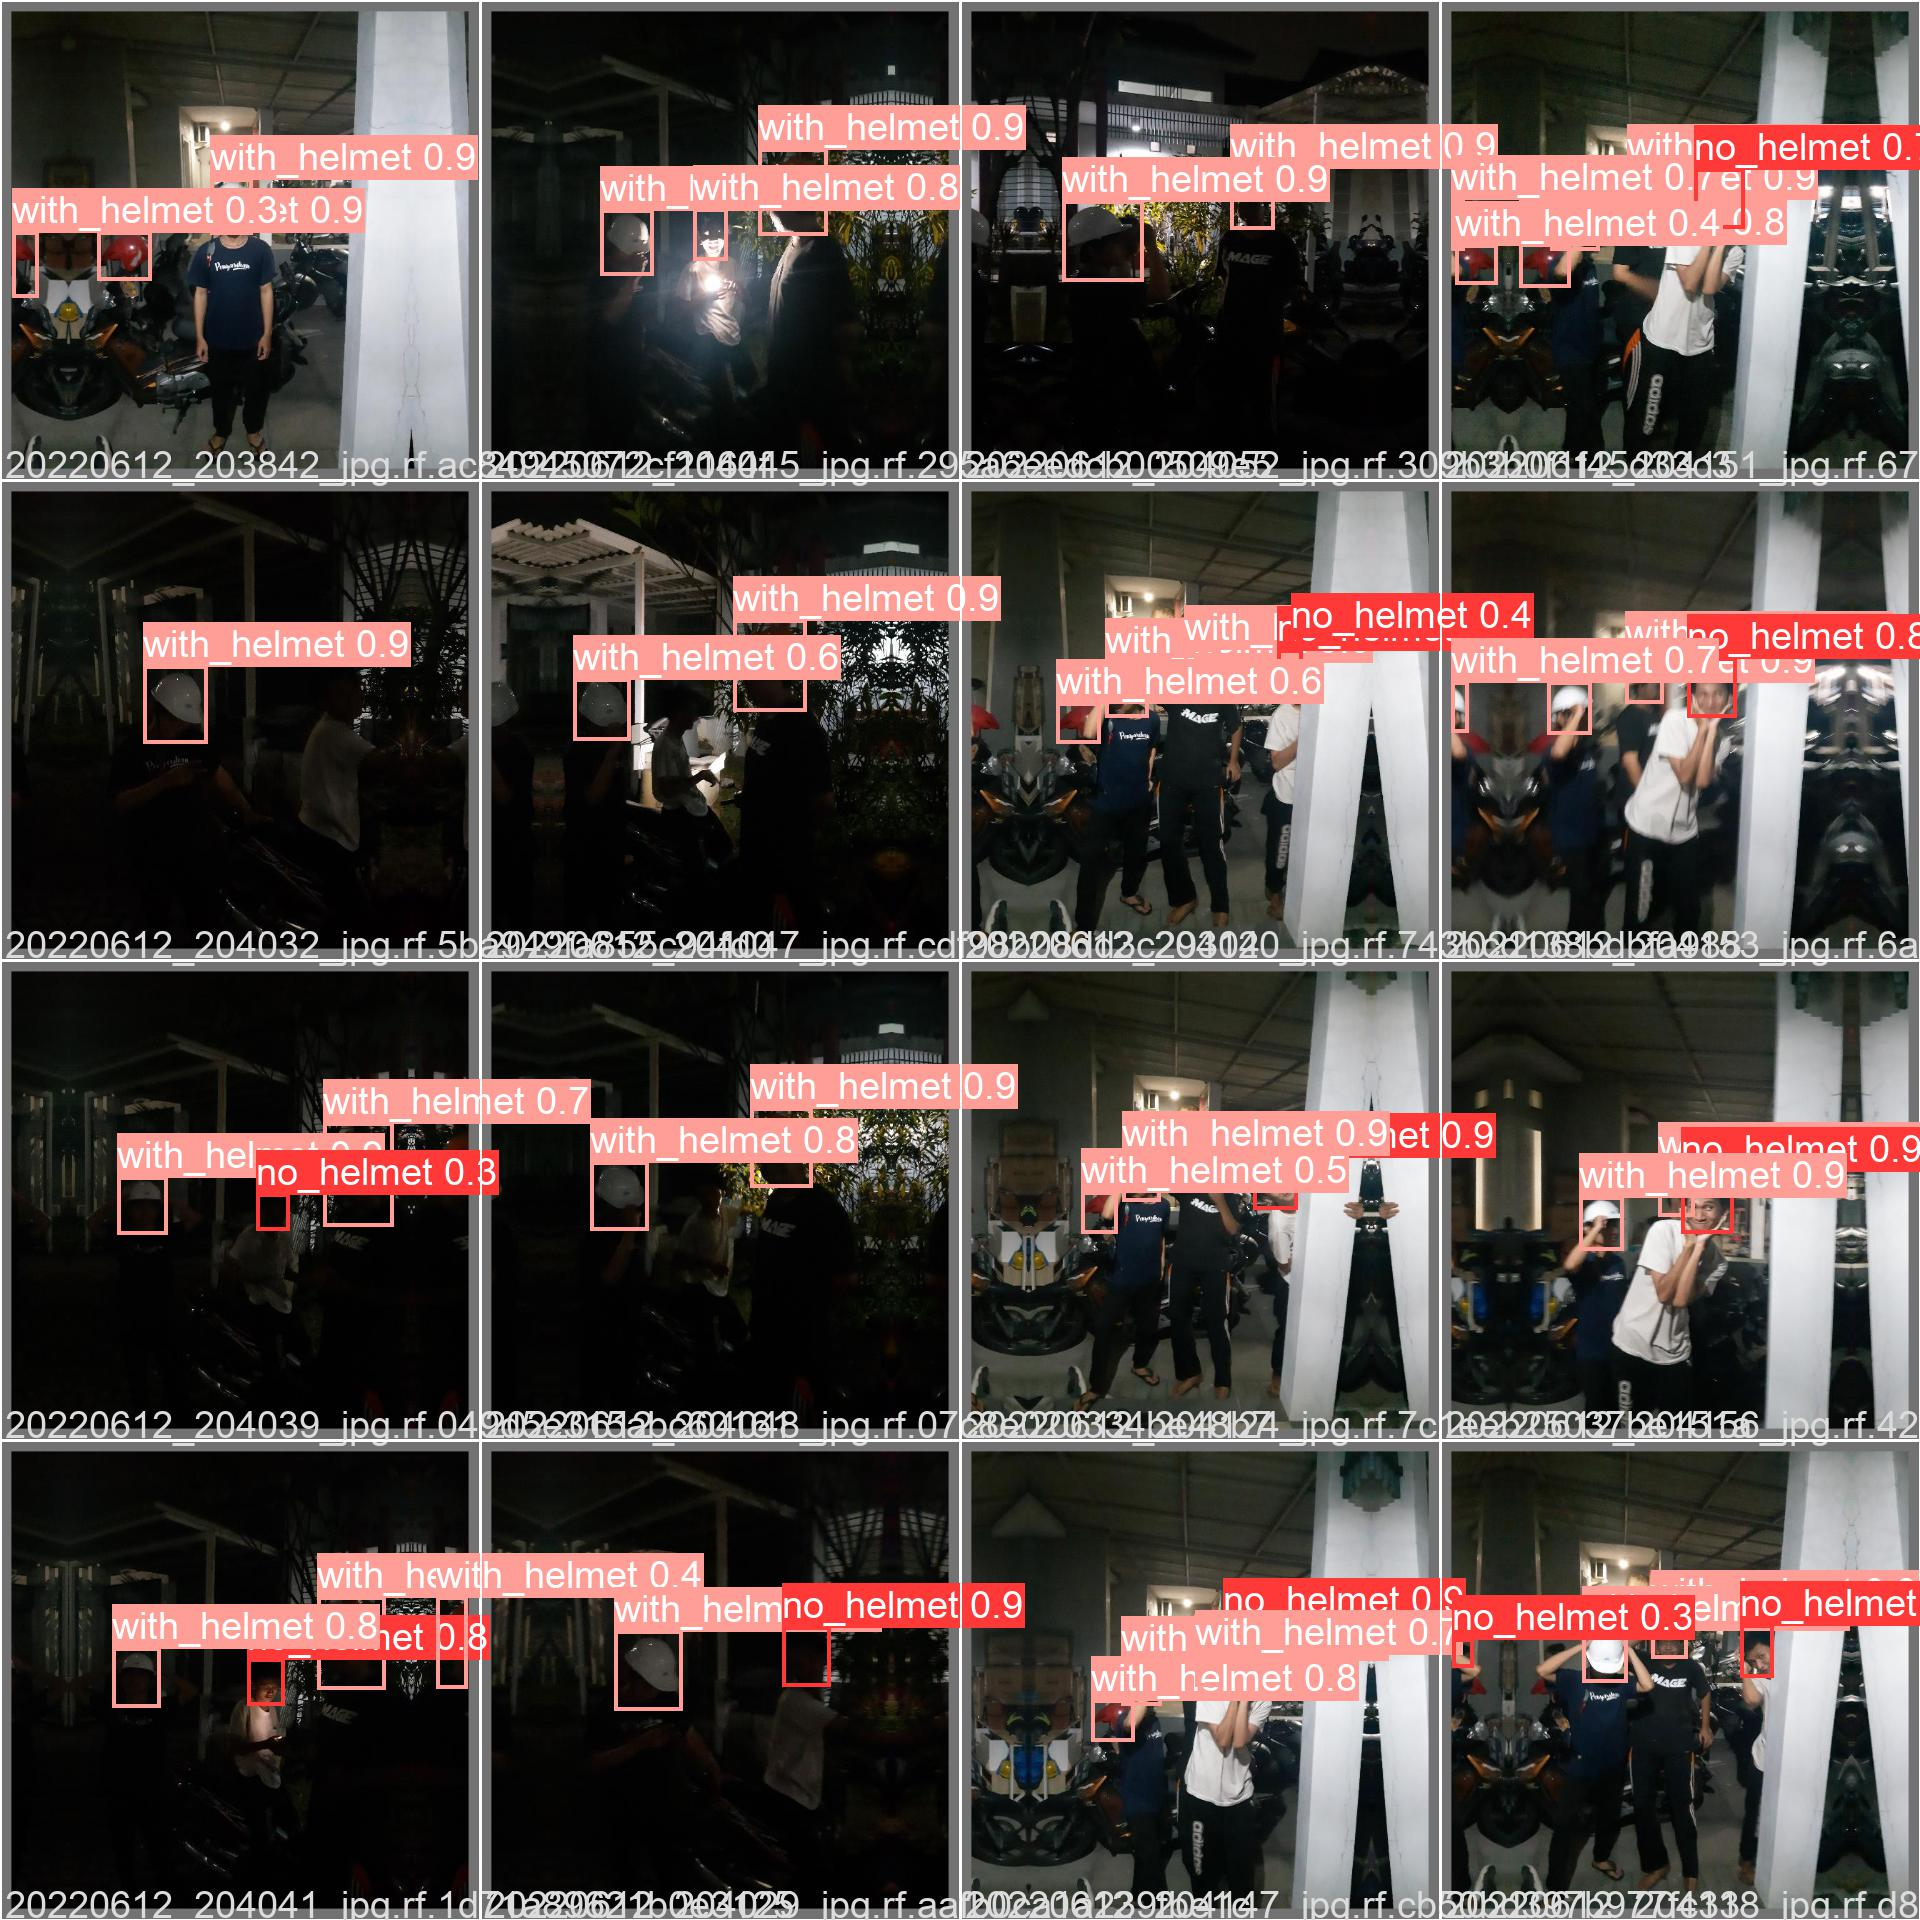
\includegraphics[scale=0.1]{gambar/train_v2_val/low_ligjt/yolosmall/low_light_val_batch0_pred.jpg}
  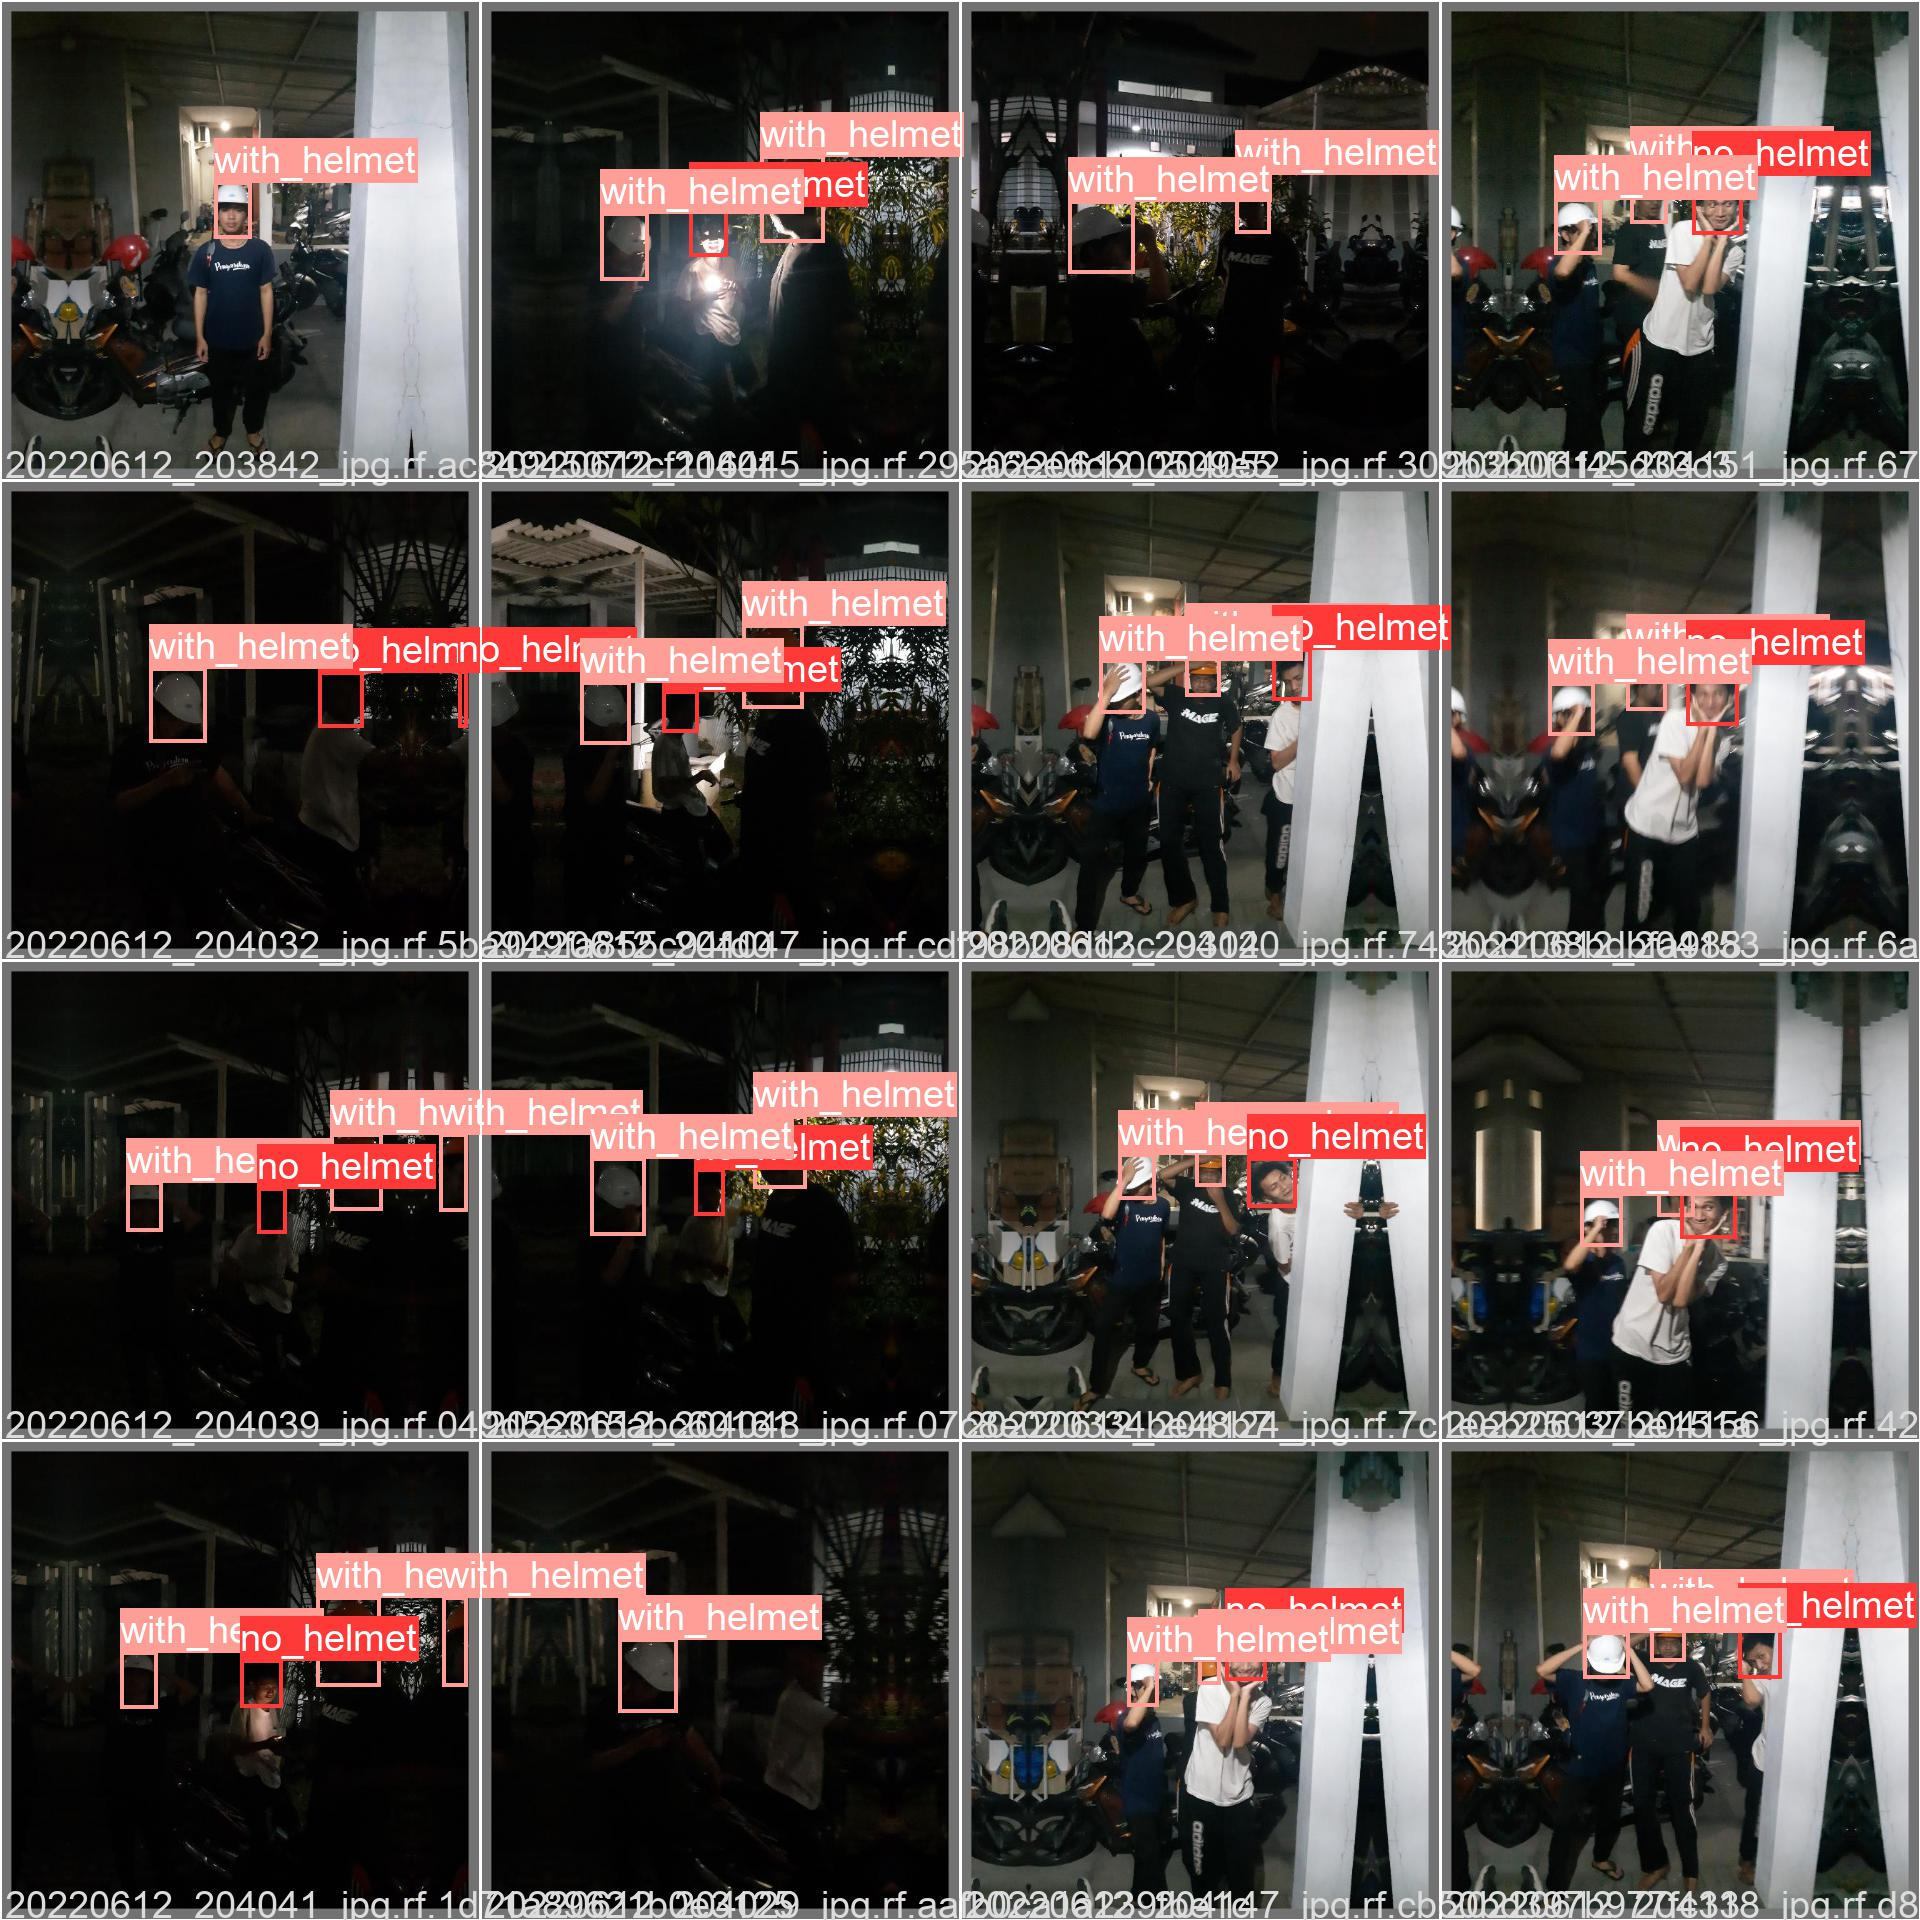
\includegraphics[scale=0.1]{gambar/train_v2_val/low_ligjt/yolosmall/lowlight_val_batch0_labels.jpg}
  \caption{Hasil Prediksi dengan Anotasi Asli Pada Keadaan dengan Pretrained YOLOvs}
  % \label{fig:labelbaru}  
\end{figure}

\subsubsection{\emph{Pretrained} YOLOv5m}
\label{subsubsec:lowlight_yolov5m}

\par Dilakukan pengujian kecerahan rendah dengan menggunakan bobot yang di-\emph{train} menggunakan bobot
pretrain COCO untuk varian \emph{medium}. Didapatkan rata - rata presisi untuk semua kelas 0.833 dan \emph{recall} untuk semua
kelas 0.831. Didapati hasil \emph{precision} dan \emph{recall} untuk kelas \emph{no\textunderscore helm} ,yang biasanya
memiliki nilai yang kurang bagus pada varian bobot nano , mendapatkan nilai 1 dan 0.68 yang dimana lebih bagus.

\begin{longtable}{|c|c|c|c|}
  \caption{Hasil Validasi Pada Tingkat Kecerahan Rendah dengan \emph{Pretrained YOLOv5m}}
  \label{tb:validasitingkatacerahrendah_yolov5m}\\
  \hline
  % \rowcolor[HTML]{C0C0C0}
  \textbf{\emph{Class} }                     & \textbf{\emph{Precision}}  & \textbf{\emph{Recall}} & \textbf{\emph{mAP@.5}}\\
  \hline
  all                                                 & 0.833          & 0.831       & 0.893         \\
  no\textunderscore helmet                            & 1              & 0.68        & 0.814         \\
  with\textunderscore helmet                          & 0.666          & 0.982       & 0.973         \\
  \hline
\end{longtable}

\begin{figure}[ht]
  \centering
  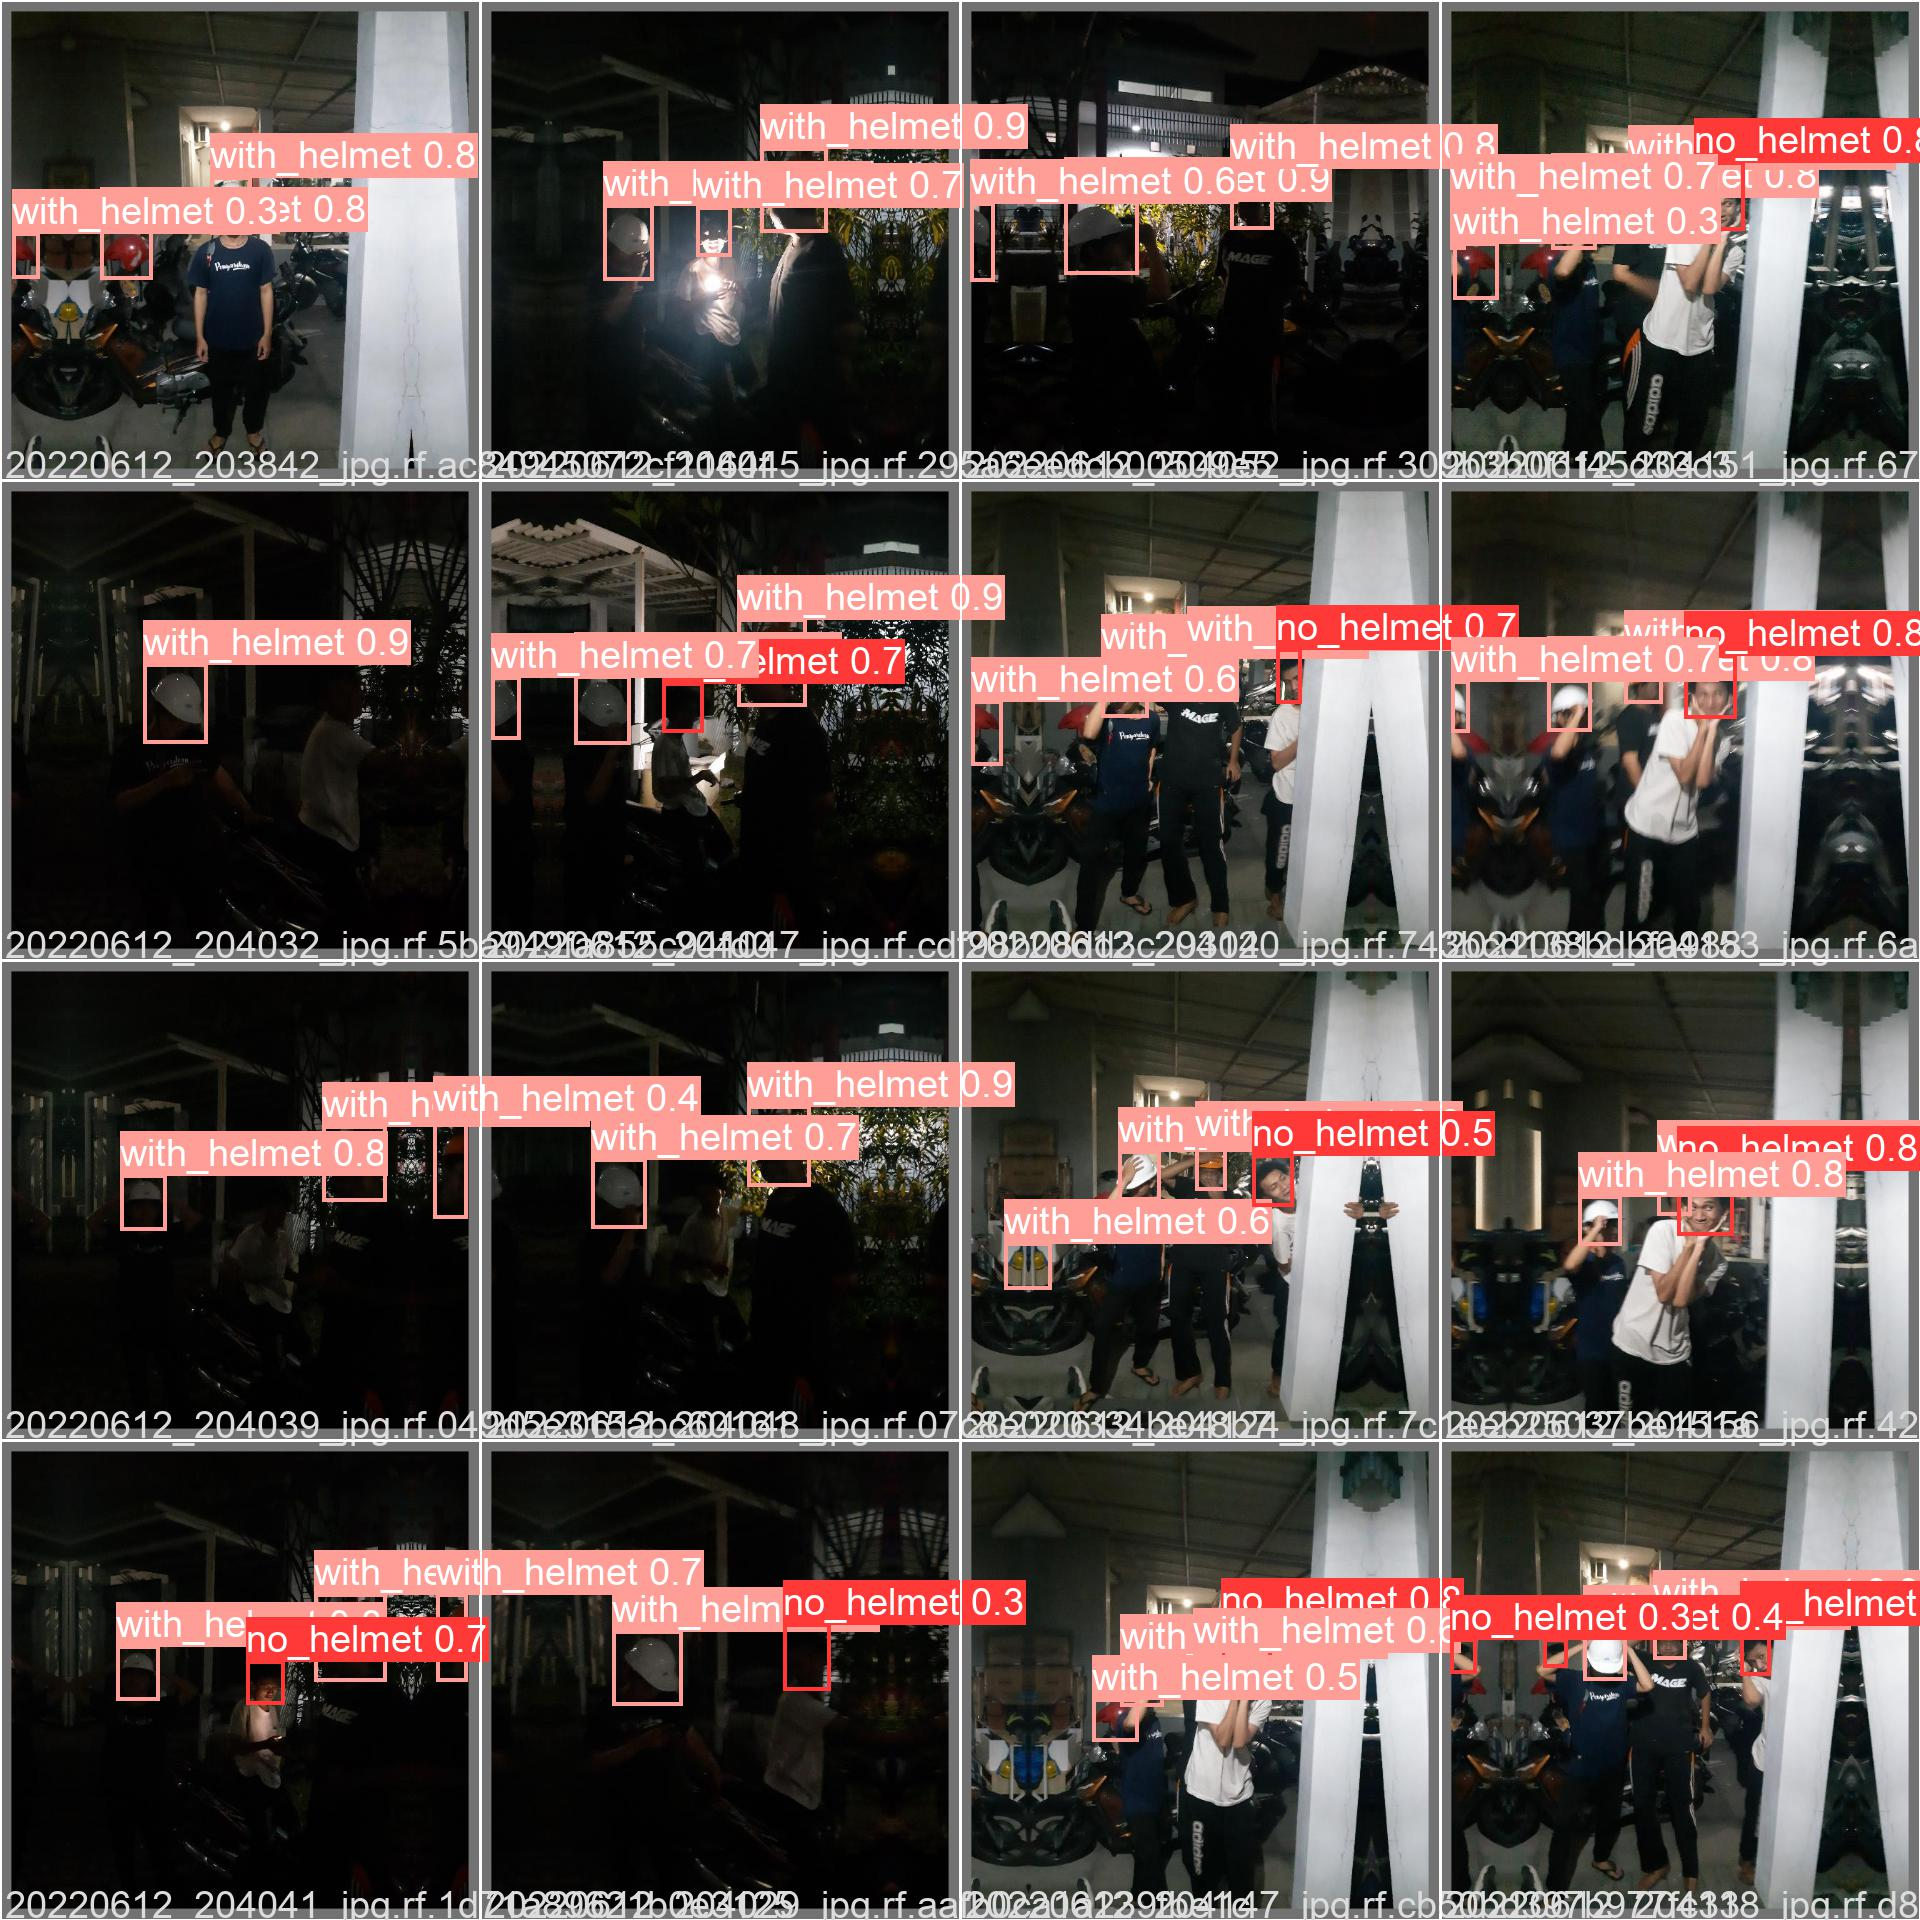
\includegraphics[scale=0.1]{gambar/train_v2_val/low_ligjt/yolomedium/val_batch0_pred.jpg}
  \includegraphics[scale=0.1]{gambar/train_v2_val/low_ligjt/yolomedium/val_batch0_labels.jpg}
  \caption{Hasil Prediksi dengan Anotasi Asli Pada Keadaan dengan Pretrained YOLOv5m}
  % \label{fig:labelbaru}  
\end{figure}

\subsubsection{\emph{Pretrained} YOLOv5l}
\label{subsubsec:lowlight_yolov5l}

\par Dilakukan pengujian kecerahan rendah dengan menggunakan bobot yang di-\emph{train} menggunakan bobot
pretrain COCO untuk varian \emph{large}. Didapatkan rata - rata presisi untuk semua kelas 0.811 dan \emph{recall} untuk semua
kelas 0.765. Didapati hasil \emph{precision} dan \emph{recall} untuk kelas \emph{no\textunderscore helm} yang mengalami penurunan dibanding
menggunakan variant \emph{medium} yaitu 0.914 untuk \emph{precision} dan 0.6 untuk \emph{recall}. Selain itu untuk
\emph{inference time} nya tentu saja mengalami kenaikan dibandingan dengan varian - varian sebelumnya yang lebih kecil.

\begin{longtable}{|c|c|c|c|}
  \caption{Hasil Validasi Pada Tingkat Kecerahan Rendah dengan \emph{Pretrained YOLOv5l}}
  \label{tb:validasitingkatacerahrendah_yolov5l}\\
  \hline
  % \rowcolor[HTML]{C0C0C0}
  \textbf{\emph{Class} }                     & \textbf{\emph{Precision}}  & \textbf{\emph{Recall}} & \textbf{\emph{mAP@.5}}\\
  \hline
  all                                                 & 0.811          & 0.765       & 0.893         \\
  no\textunderscore helmet                            & 0.914          & 0.6         & 0.724         \\
  with\textunderscore helmet                          & 0.708          & 0.93        & 0.931         \\
  \hline
\end{longtable}

\begin{figure}[ht]
  \centering
  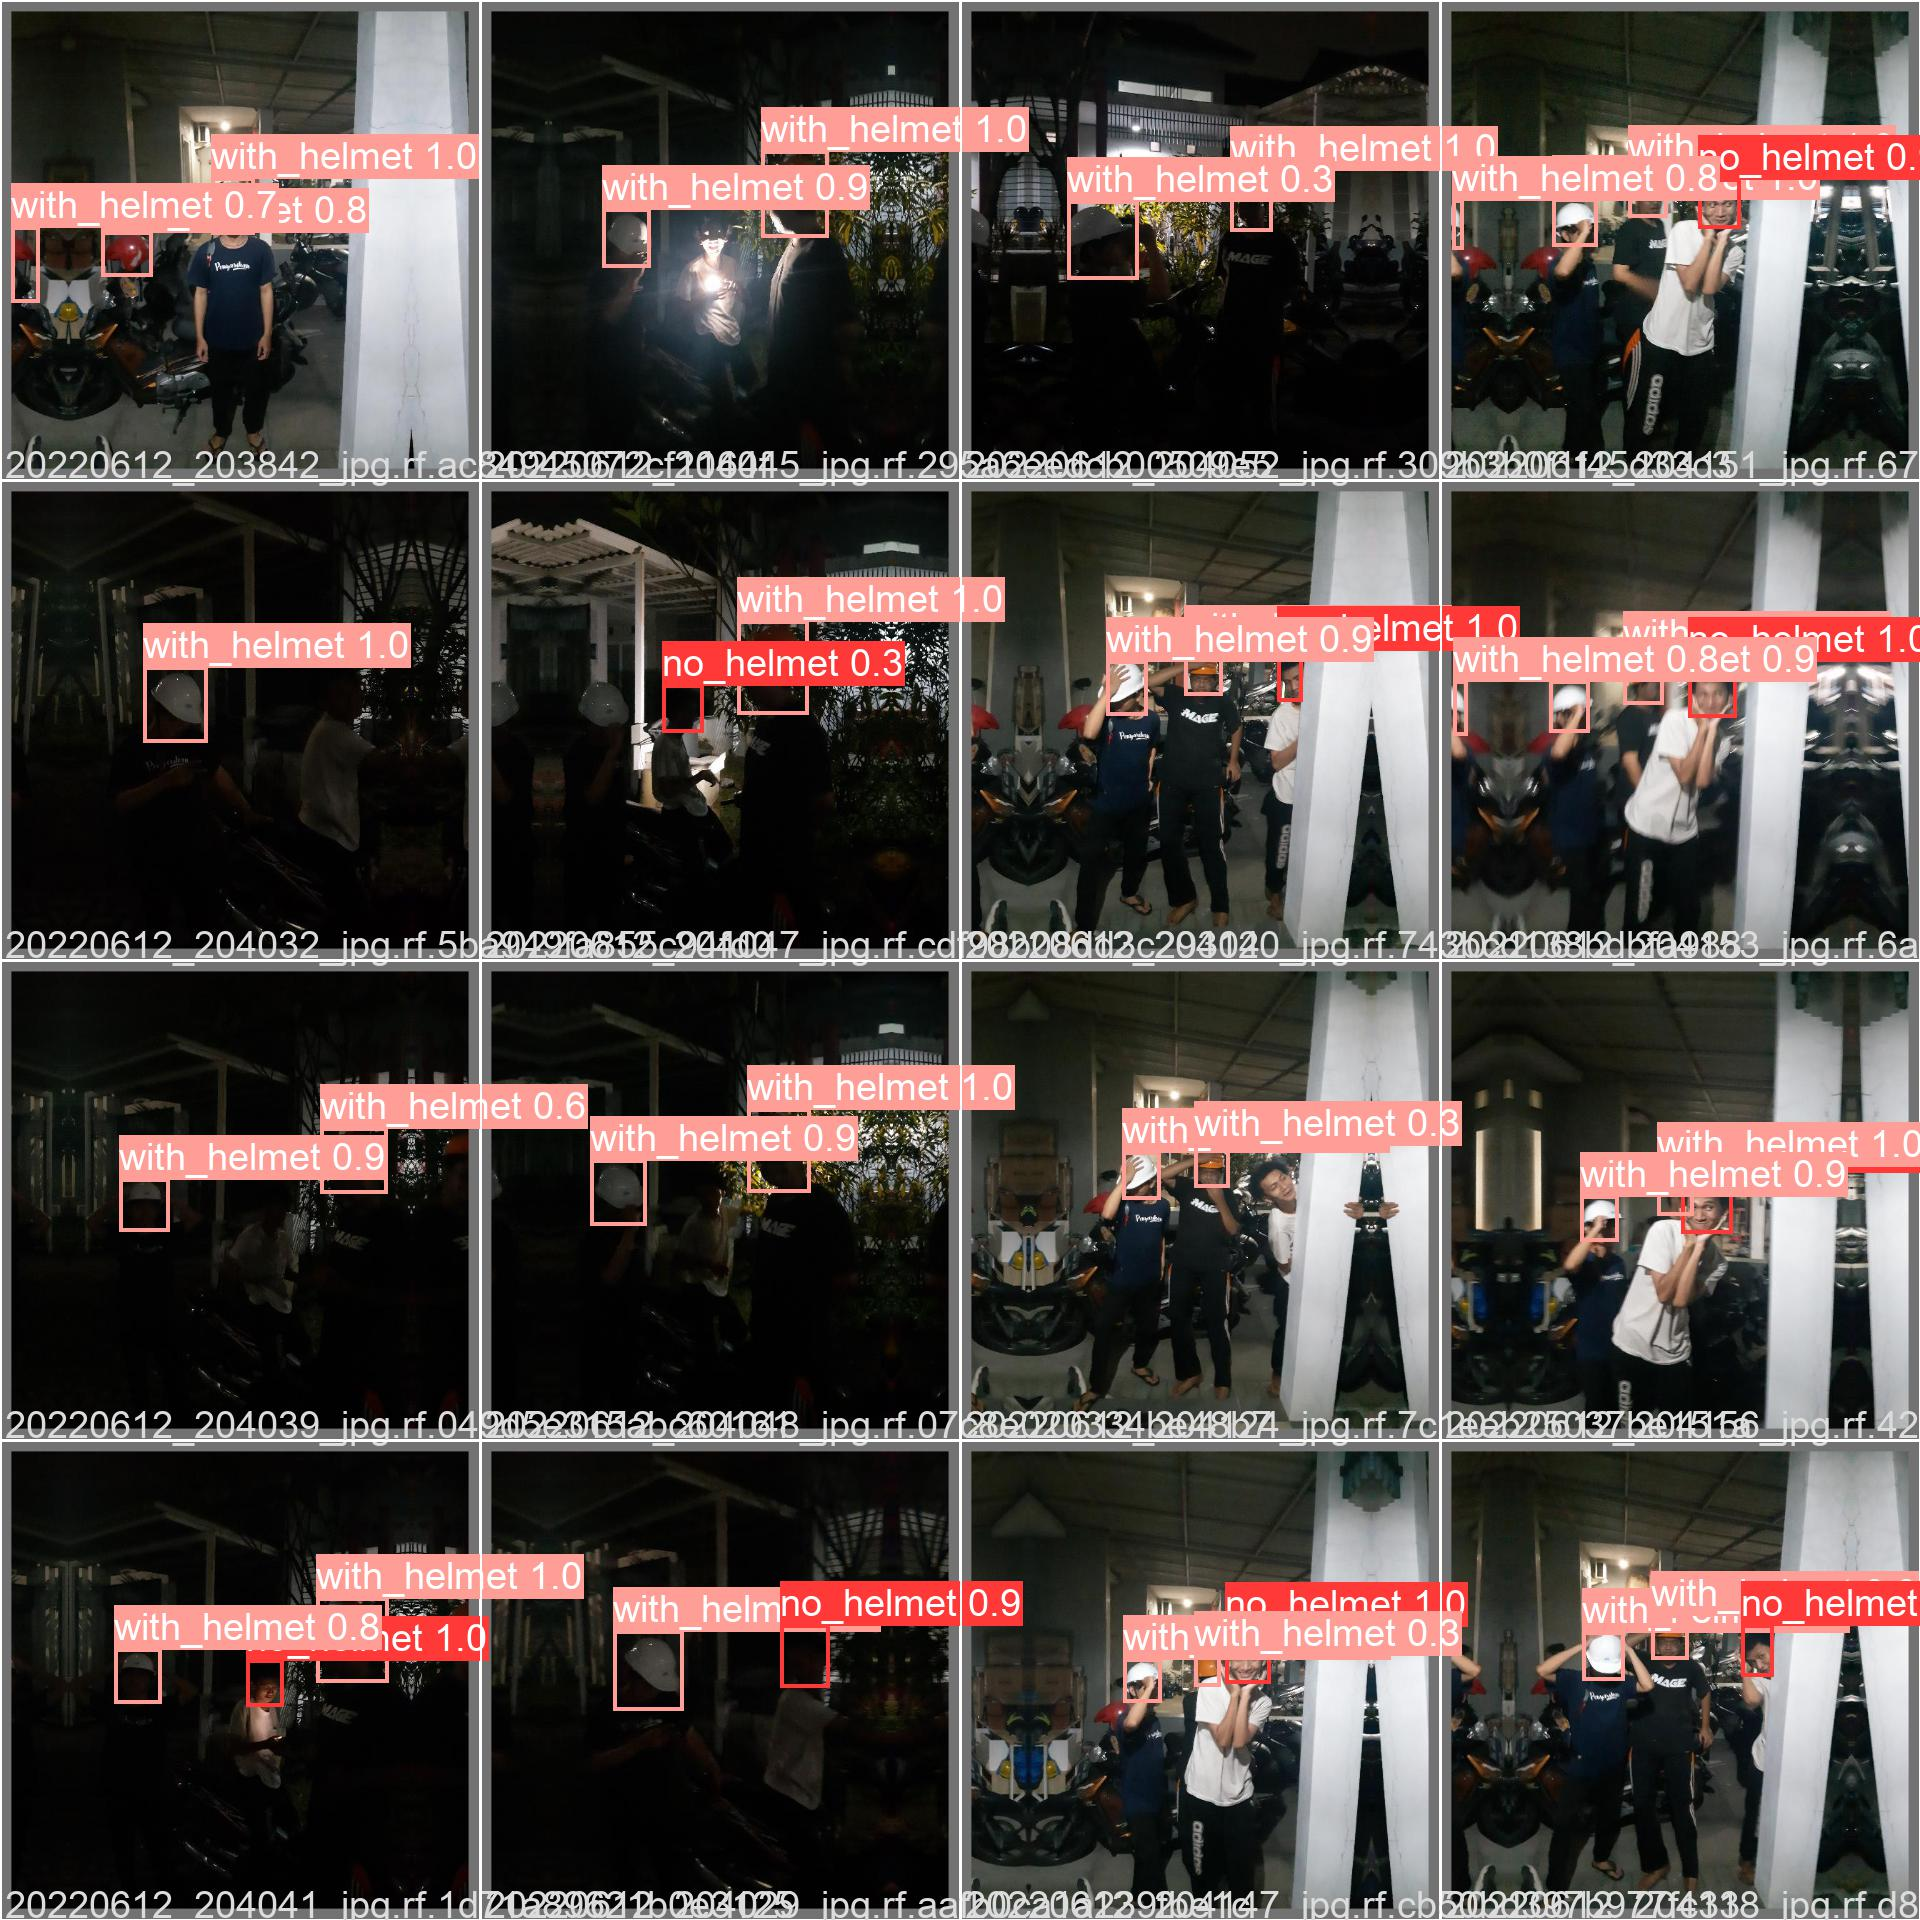
\includegraphics[scale=0.1]{gambar/train_v2_val/low_ligjt/yololarge/val_batch0_pred.jpg}
  \includegraphics[scale=0.1]{gambar/train_v2_val/low_ligjt/yololarge/val_batch0_labels.jpg}
  \caption{Hasil Prediksi dengan Anotasi Asli Pada Keadaan dengan Pretrained YOLOv5m}
  % \label{fig:labelbaru}  
\end{figure}

\subsection{Pengujian Pada Tingkat Kecerahan Rendah dengan \emph{Weight} Murni Deteksi Helm Keselamatan Kerja}
\label{subsec:lowlight_pure}

\par Berikut merupakan pemaparan hasil validasi menggunakan data validasi pada keadaan minim pencahayaan menggunakan
\emph{weight} yang merupakan hasil \emph{train} dari dataset Deteksi Helm Keselamatan Kerja tanpa menggunakan \emph{pretrained weight}.
Hasil \emph{train} tanpa menggunakan \emph{pretrain weight} ini selanjutkan akan disebut sebagai \emph{"Hedec"}.


\subsubsection{\emph{Hedec Nano}}
\label{subsubsec:lowlight_hedecN}

\par Dilakukan pengujian kecerahan rendah dengan menggunakan bobot yang di-\emph{train} tanpa menggunakan bobot
pretrain COCO tetapi konfigurasi modelnya dibuat serupa dengan konfigurasi YOLOv5n. 
Didapatkan rata - rata presisi untuk semua kelas 0.659   dan \emph{recall} untuk semuakelas 0.696.
\par Didapati pada gambar dengan tingkat kecerahan sangat rendah, tidak terdeteksi untuk kedua kelas 
sama sekali dan juga \emph{miss detect} untuk kepala tanpa helm dideteksi 
sebagai \emph{with\textunderscore helmet}.

\begin{longtable}{|c|c|c|c|}
  \caption{Hasil Validasi Pada Tingkat Kecerahan Rendah dengan \emph{Hedec Nano}}
  \label{tb:validasitingkatacerahrendah_hedecN}\\
  \hline
  % \rowcolor[HTML]{C0C0C0}
  \textbf{\emph{Class} }                     & \textbf{\emph{Precision}}  & \textbf{\emph{Recall}} & \textbf{\emph{mAP@.5}}\\
  \hline
  all                                                 & 0.659          & 0.696       & 0.731         \\
  no\textunderscore helmet                            & 0.76          & 0.55         & 0.621         \\
  with\textunderscore helmet                          & 0.558          & 0.842        & 0.842         \\
  \hline
\end{longtable}

\begin{figure}[ht]
  \centering
  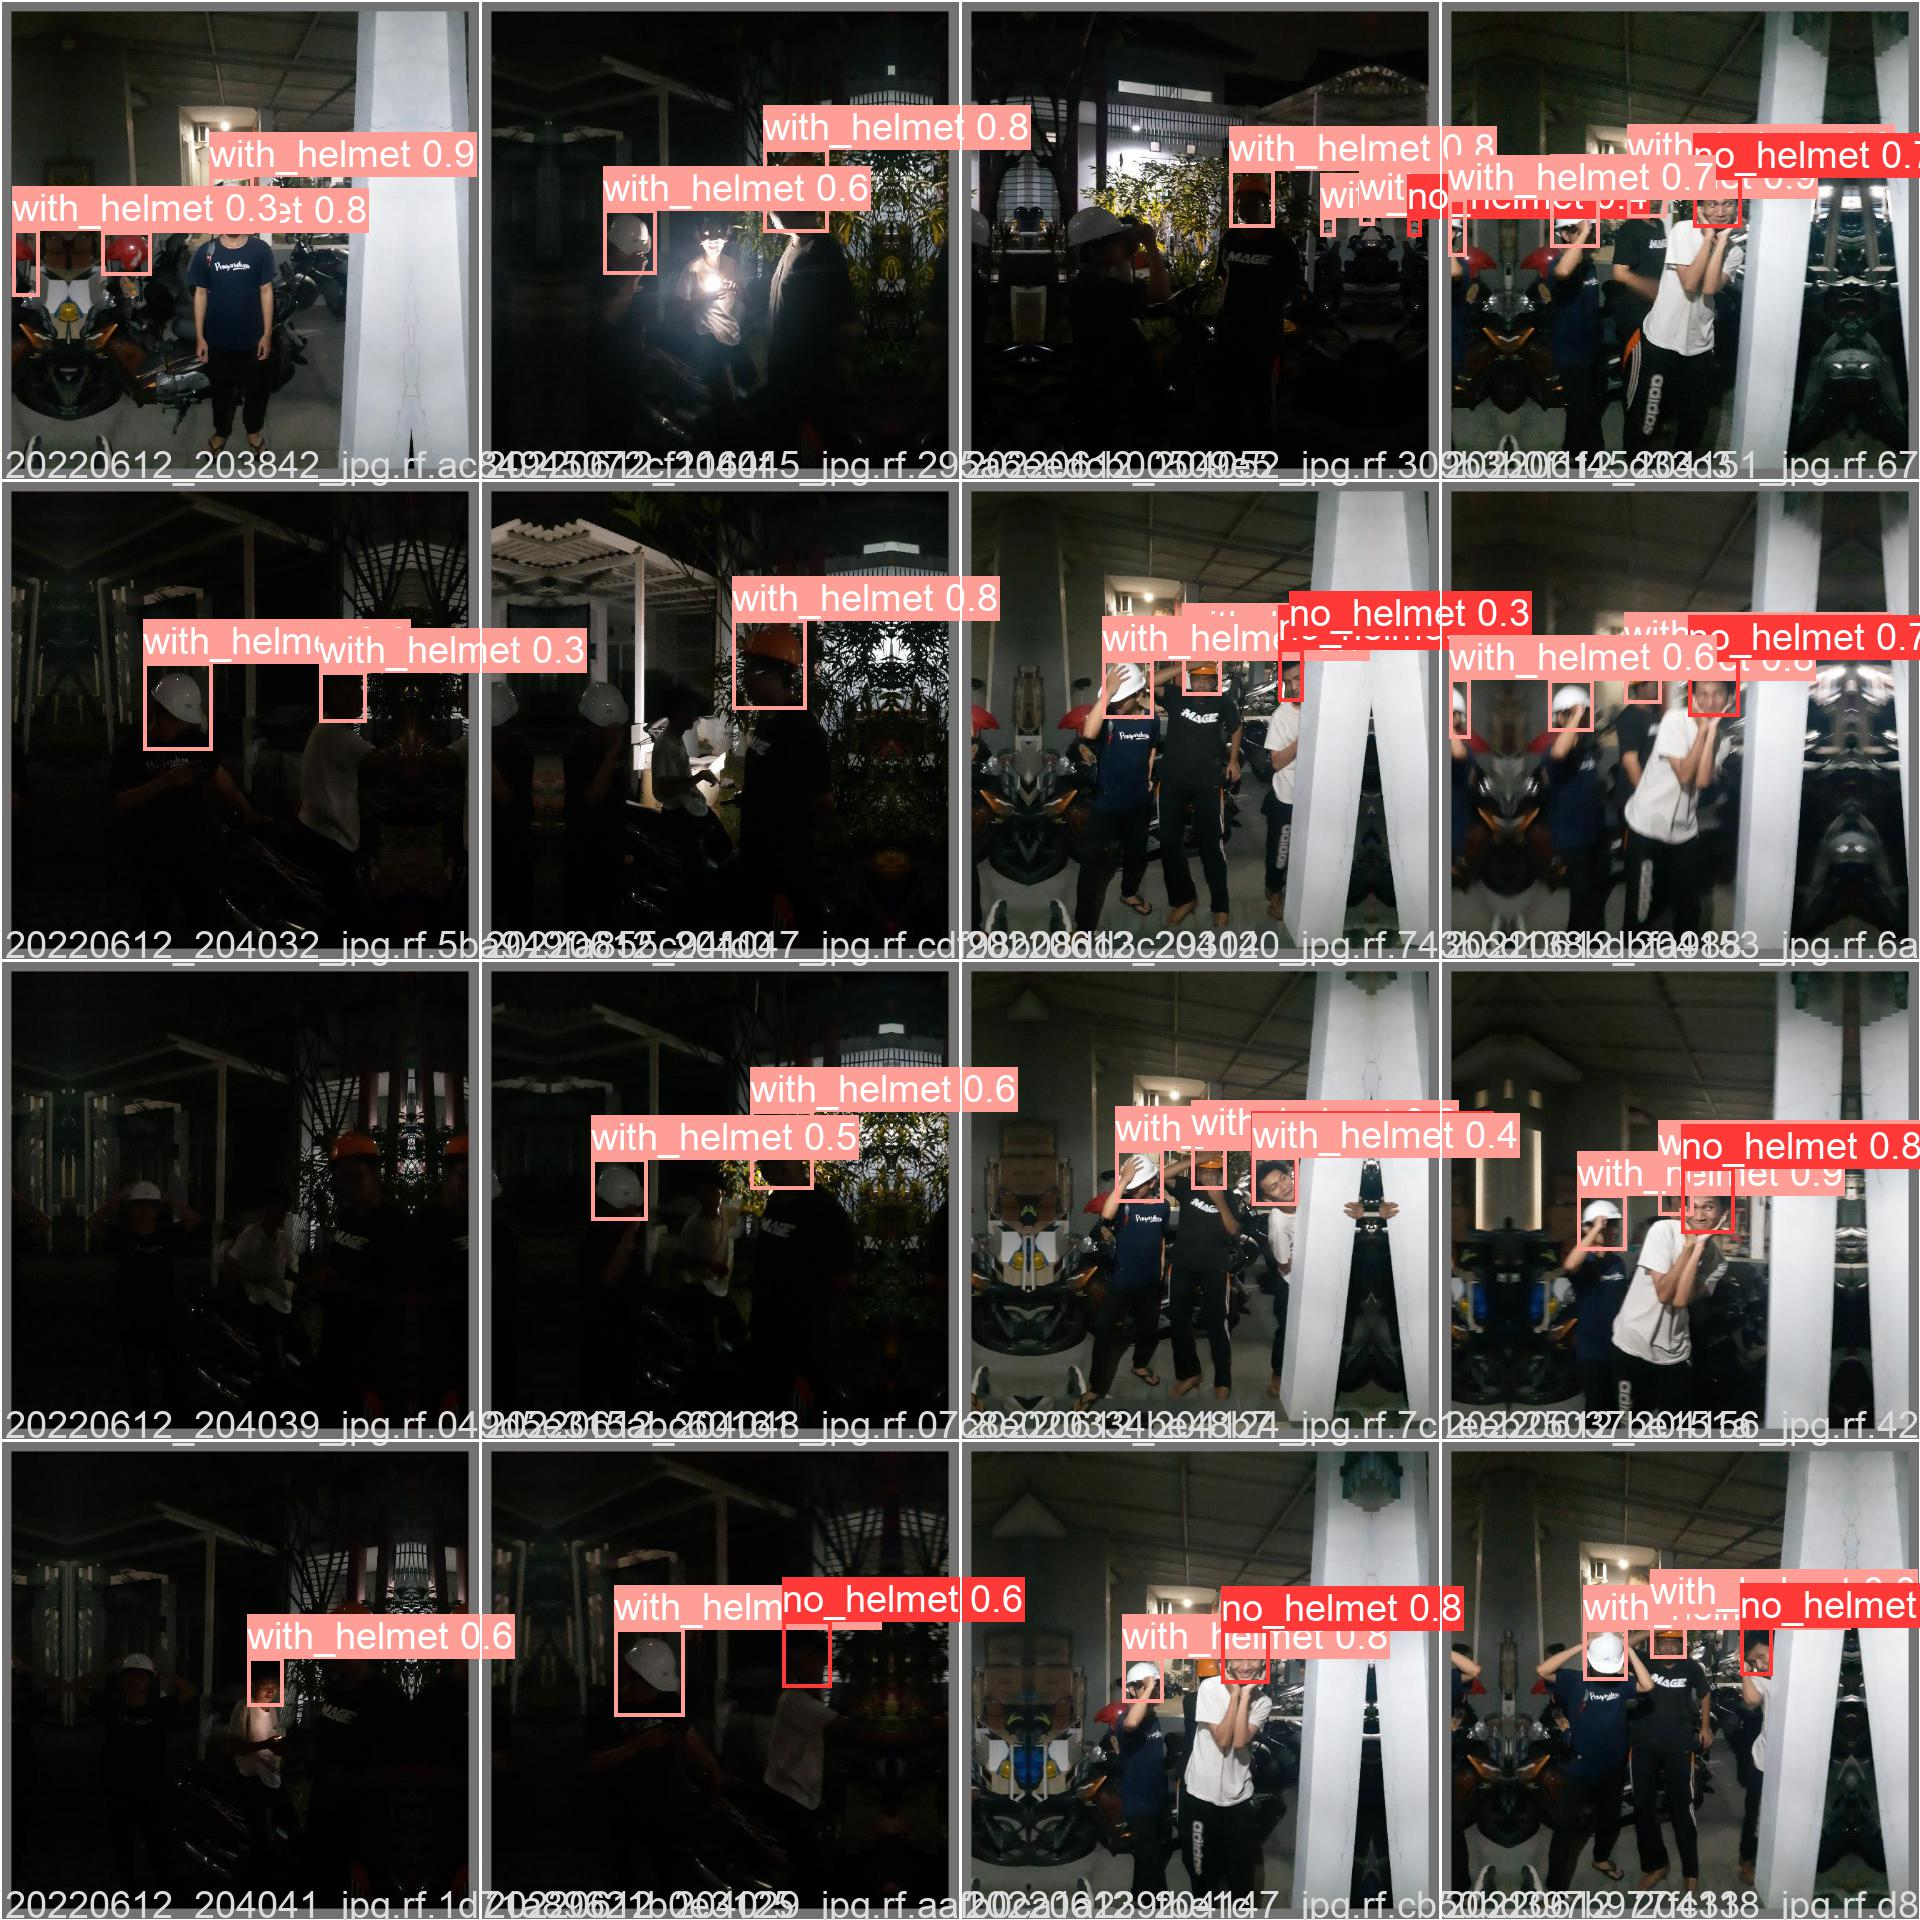
\includegraphics[scale=0.1]{gambar/train_v2_val/low_ligjt/customNano/val_batch0_pred.jpg}
  \includegraphics[scale=0.1]{gambar/train_v2_val/low_ligjt/customNano/val_batch0_labels.jpg}
  \caption{Hasil Prediksi dengan Anotasi Asli Pada Keadaan dengan \emph{Weight Hedec Nano}}
  % \label{fig:labelbaru}  
\end{figure}

\subsubsection{\emph{Hedec Small}}
\label{subsubsec:lowlight_hedecS}

\par Dilakukan pengujian kecerahan rendah dengan menggunakan bobot yang di-\emph{train} tanpa menggunakan bobot
pretrain COCO tetapi konfigurasi modelnya dibuat serupa dengan konfigurasi YOLOv5s. 
Didapatkan rata - rata presisi untuk semua kelas 0.659   dan \emph{recall} untuk semuakelas 0.696.
\par Didapati pada gambar dengan tingkat kecerahan sangat rendah, tidak terdeteksi untuk kedua kelas 
sama sekali dan juga \emph{miss detect} untuk kepala tanpa helm dideteksi 
sebagai \emph{with\textunderscore helmet}.

\begin{longtable}{|c|c|c|c|}
  \caption{Hasil Validasi Pada Tingkat Kecerahan Rendah dengan \emph{Hedec Small}}
  \label{tb:validasitingkatacerahrendah_hedecS}\\
  \hline
  % \rowcolor[HTML]{C0C0C0}
  \textbf{\emph{Class} }                     & \textbf{\emph{Precision}}  & \textbf{\emph{Recall}} & \textbf{\emph{mAP@.5}}\\
  \hline
  all                                                 & 0.706          & 0.696       & 0.731         \\
  no\textunderscore helmet                            & 0.76          & 0.55         & 0.621         \\
  with\textunderscore helmet                          & 0.558          & 0.842        & 0.842         \\
  \hline
\end{longtable}

\begin{figure}[ht]
  \centering
  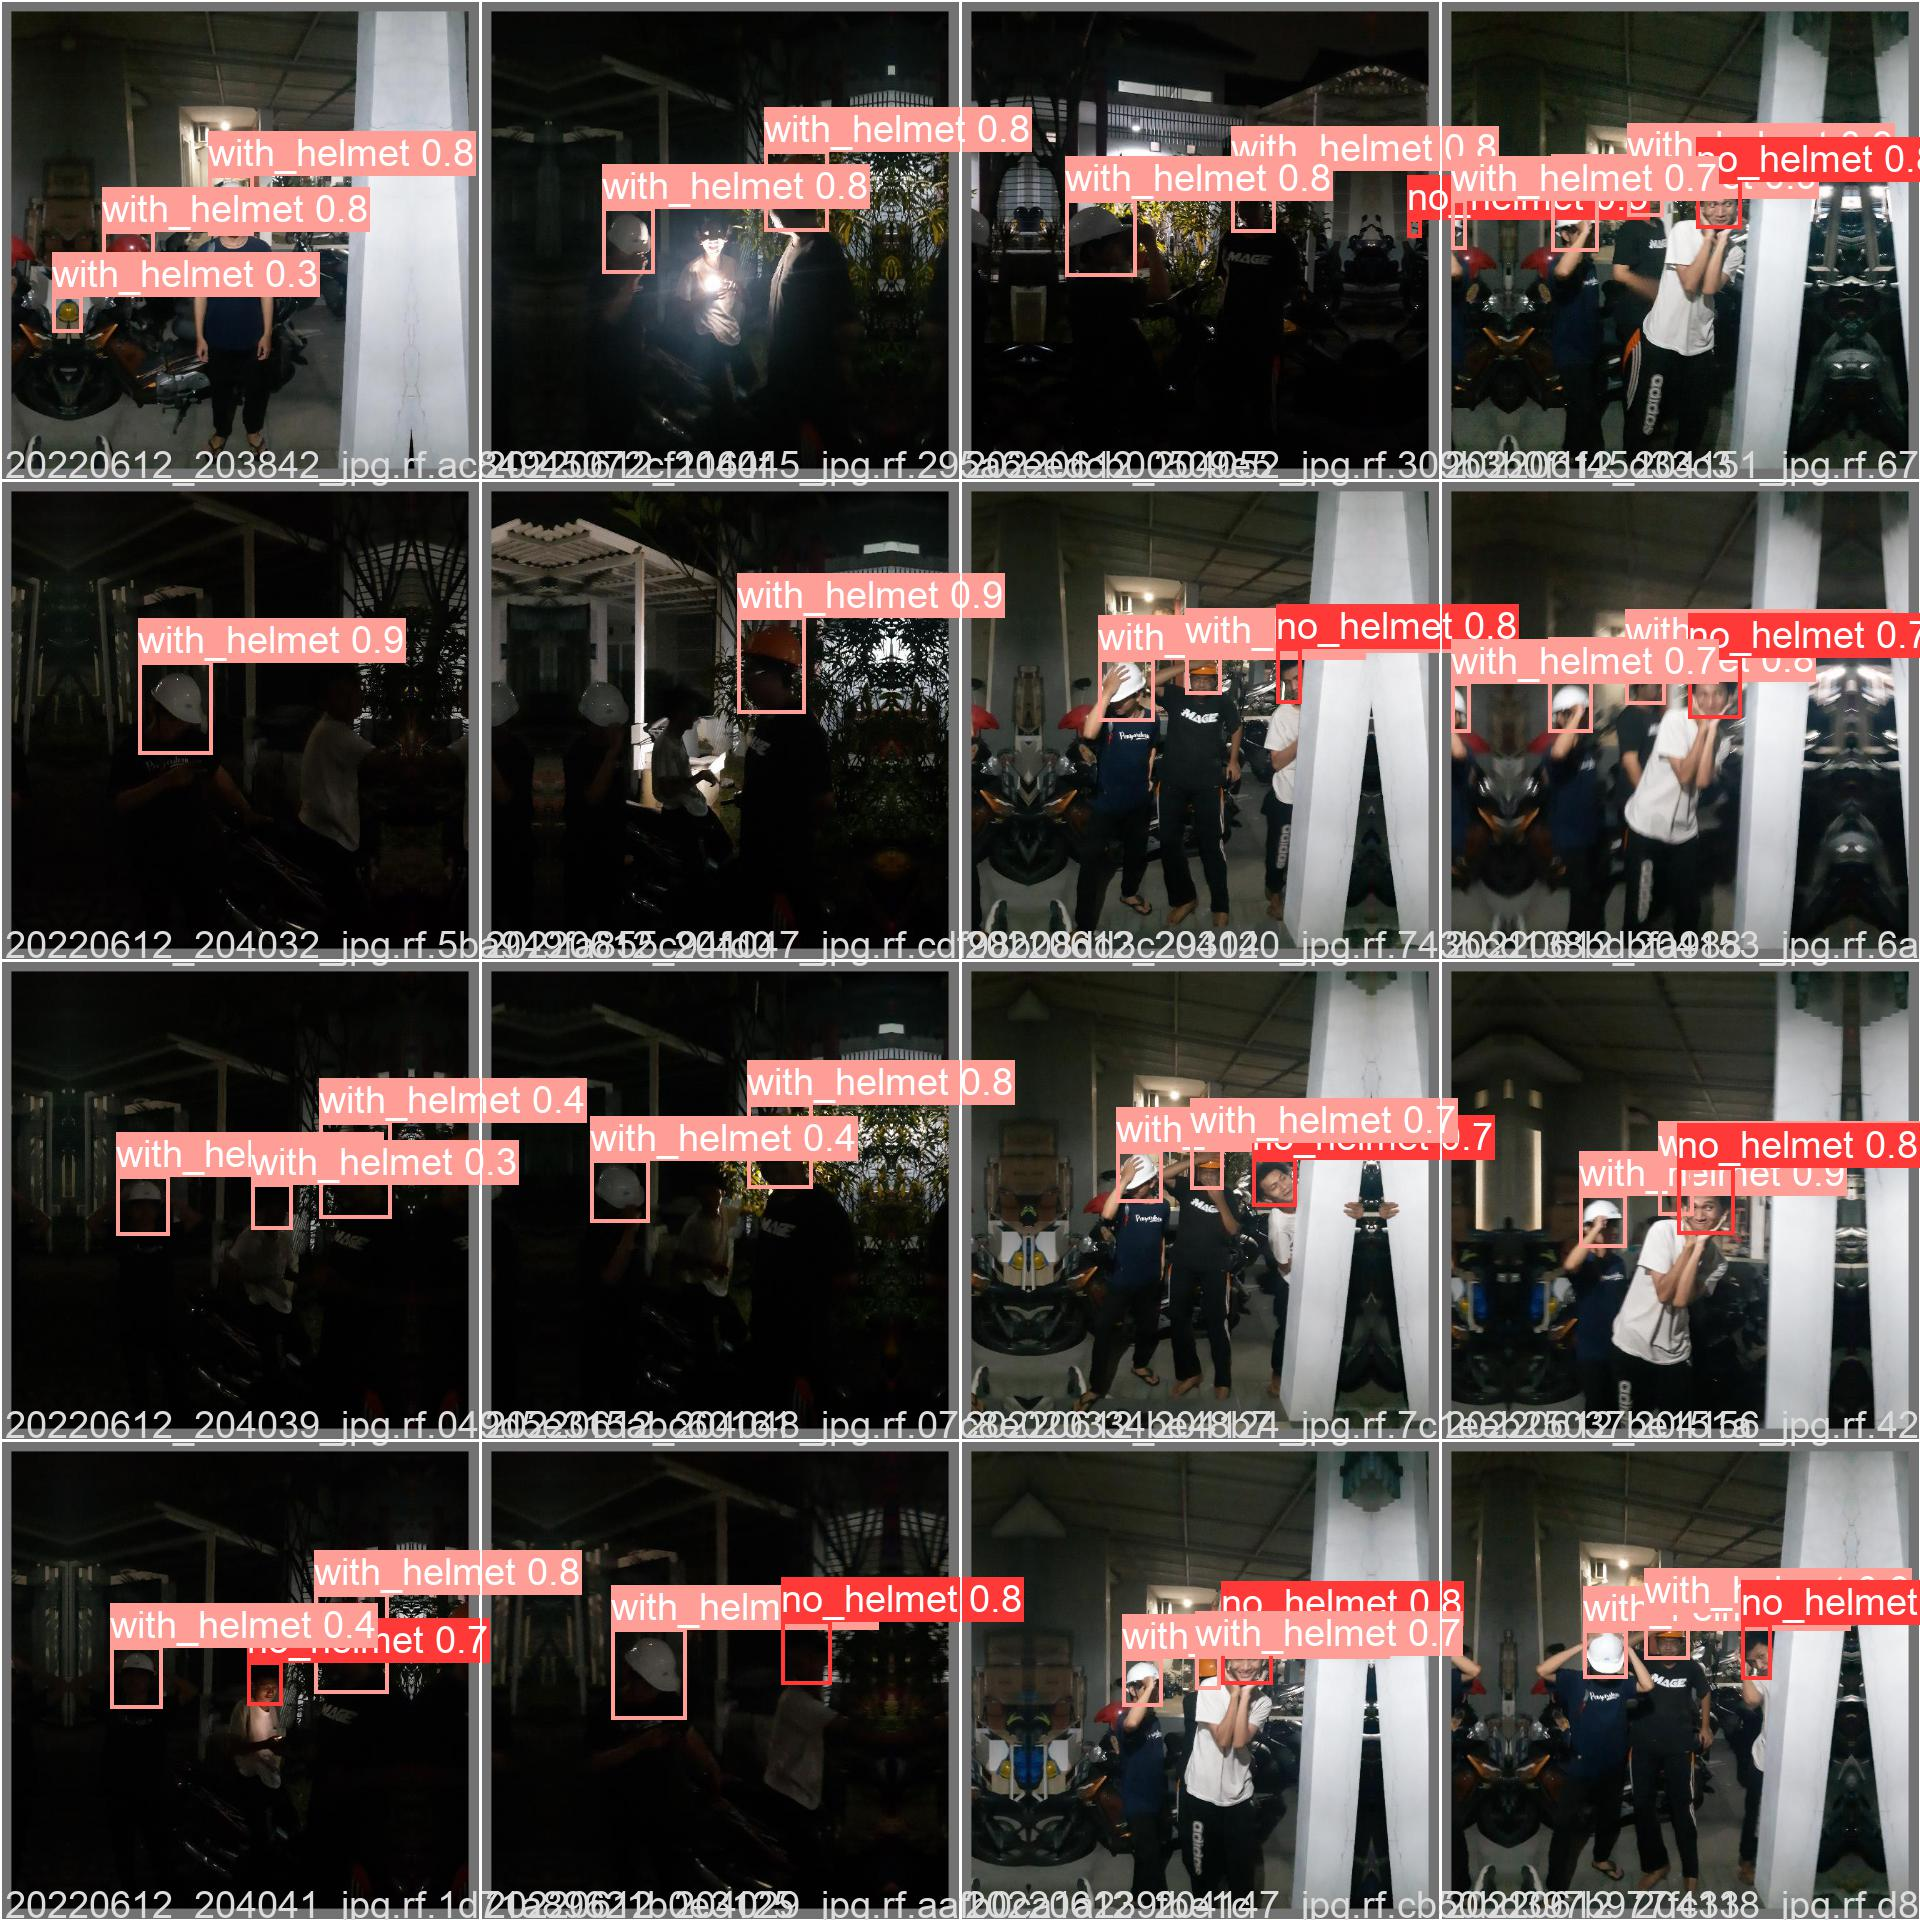
\includegraphics[scale=0.1]{gambar/train_v2_val/low_ligjt/customSmall/val_batch0_pred.jpg}
  \includegraphics[scale=0.1]{gambar/train_v2_val/low_ligjt/customSmall/val_batch0_labels.jpg}
  \caption{Hasil Prediksi dengan Anotasi Asli Pada Keadaan dengan \emph{Weight Hedec Small}}
  % \label{fig:labelbaru}  
\end{figure}

\subsubsection{\emph{Hedec Medium}}
\label{subsubsec:lowlight_hedecM}

\par Dilakukan pengujian kecerahan rendah dengan menggunakan bobot yang di-\emph{train} tanpa menggunakan bobot
pretrain COCO tetapi konfigurasi modelnya dibuat serupa dengan konfigurasi YOLOv5m. 
Didapatkan rata - rata presisi untuk semua kelas 0.731   dan \emph{recall} untuk semuakelas 0.862.
\par Didapati pada gambar dengan tingkat kecerahan sangat rendah, tidak terdeteksi untuk kedua kelas 
sama sekali dan juga \emph{miss detect} untuk kepala tanpa helm dideteksi 
sebagai \emph{with\textunderscore helmet}.

\begin{longtable}{|c|c|c|c|}
  \caption{Hasil Validasi Pada Tingkat Kecerahan Rendah dengan \emph{Hedec Medium}}
  \label{tb:validasitingkatacerahrendah_hedecM}\\
  \hline
  % \rowcolor[HTML]{C0C0C0}
  \textbf{\emph{Class} }                     & \textbf{\emph{Precision}}  & \textbf{\emph{Recall}} & \textbf{\emph{mAP@.5}}\\
  \hline
  all                                                 & 0.731          & 0.862       & 0.827         \\
  no\textunderscore helmet                            & 0.799          & 0.793       & 0.757         \\
  with\textunderscore helmet                          & 0.663          & 0.93        & 0.897         \\
  \hline
\end{longtable}

\begin{figure}[ht]
  \centering
  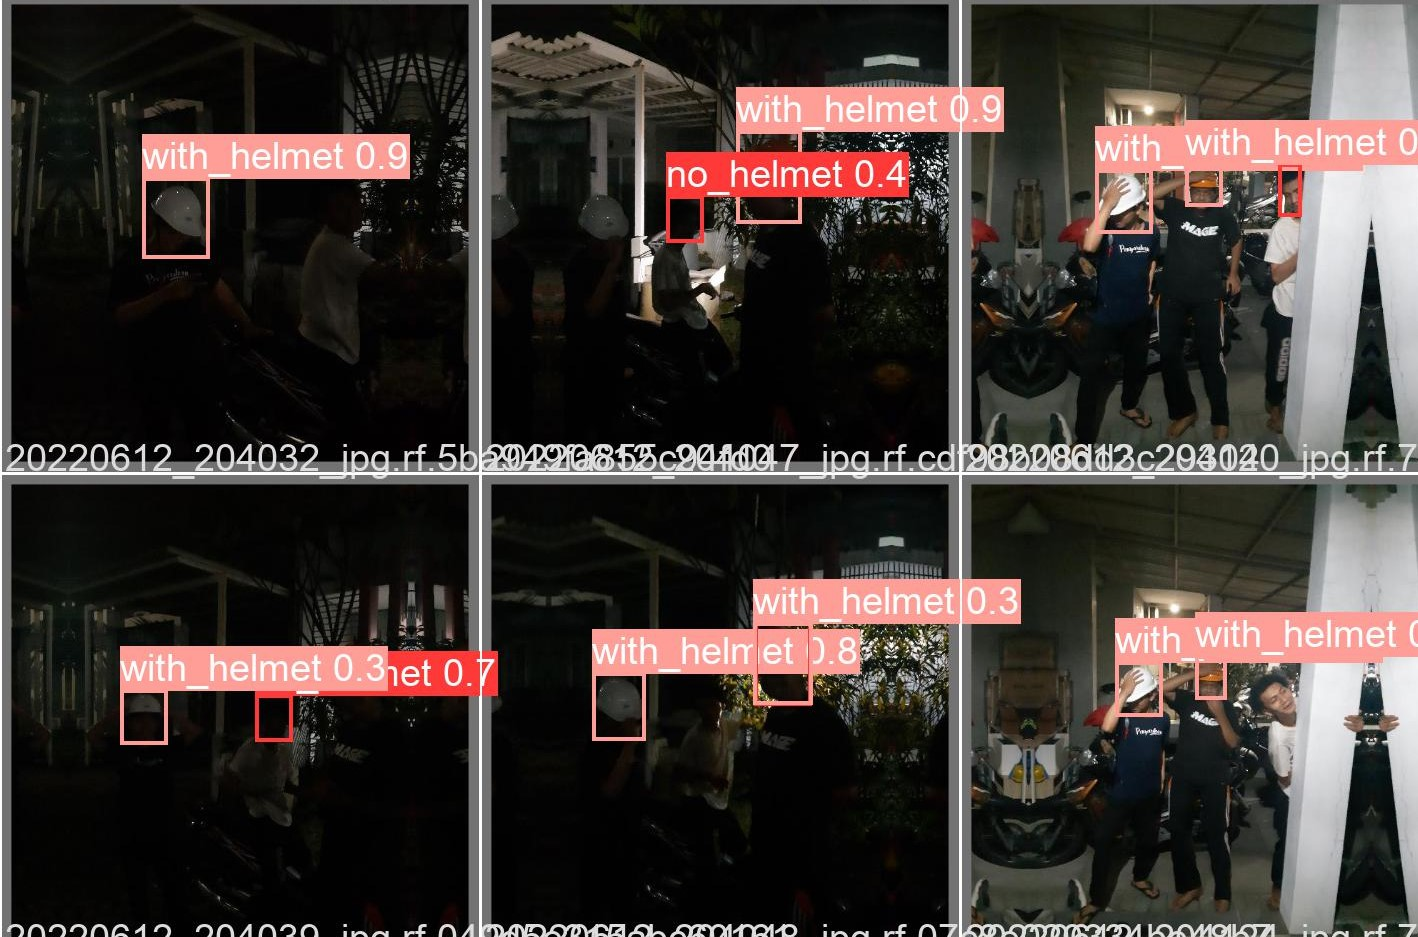
\includegraphics[scale=0.1]{gambar/train_v2_val/low_ligjt/customMedium/val_batch0_pred.jpg}
  \includegraphics[scale=0.1]{gambar/train_v2_val/low_ligjt/customMedium/val_batch0_labels.jpg}
  \caption{Hasil Prediksi dengan Anotasi Asli Pada Keadaan dengan \emph{Weight Hedec Medium}}
  % \label{fig:labelbaru}  
\end{figure}

\subsubsection{\emph{Hedec large}}
\label{subsubsec:lowlight_hedecL}

\par Dilakukan pengujian kecerahan rendah dengan menggunakan bobot yang di-\emph{train} tanpa menggunakan bobot
pretrain COCO tetapi konfigurasi modelnya dibuat serupa dengan konfigurasi YOLOv5l. 
Didapatkan rata - rata presisi untuk semua kelas 0.731   dan \emph{recall} untuk semuakelas 0.862.
\par Didapati pada gambar dengan tingkat kecerahan sangat rendah, tidak terdeteksi untuk kedua kelas 
sama sekali dan juga \emph{miss detect} untuk kepala tanpa helm dideteksi 
sebagai \emph{with\textunderscore helmet}.

\begin{longtable}{|c|c|c|c|}
  \caption{Hasil Validasi Pada Tingkat Kecerahan Rendah dengan \emph{Hedec Large}}
  \label{tb:validasitingkatacerahrendah_hedecL}\\
  \hline
  % \rowcolor[HTML]{C0C0C0}
  \textbf{\emph{Class} }                     & \textbf{\emph{Precision}}  & \textbf{\emph{Recall}} & \textbf{\emph{mAP@.5}}\\
  \hline
  all                                                 & 0.743          & 0.755       & 0.789         \\
  no\textunderscore helmet                            & 0.85           & 0.65       & 0.733         \\
  with\textunderscore helmet                          & 0.663          & 0.86        & 0.845         \\
  \hline
\end{longtable}

\begin{figure}[ht]
  \centering
  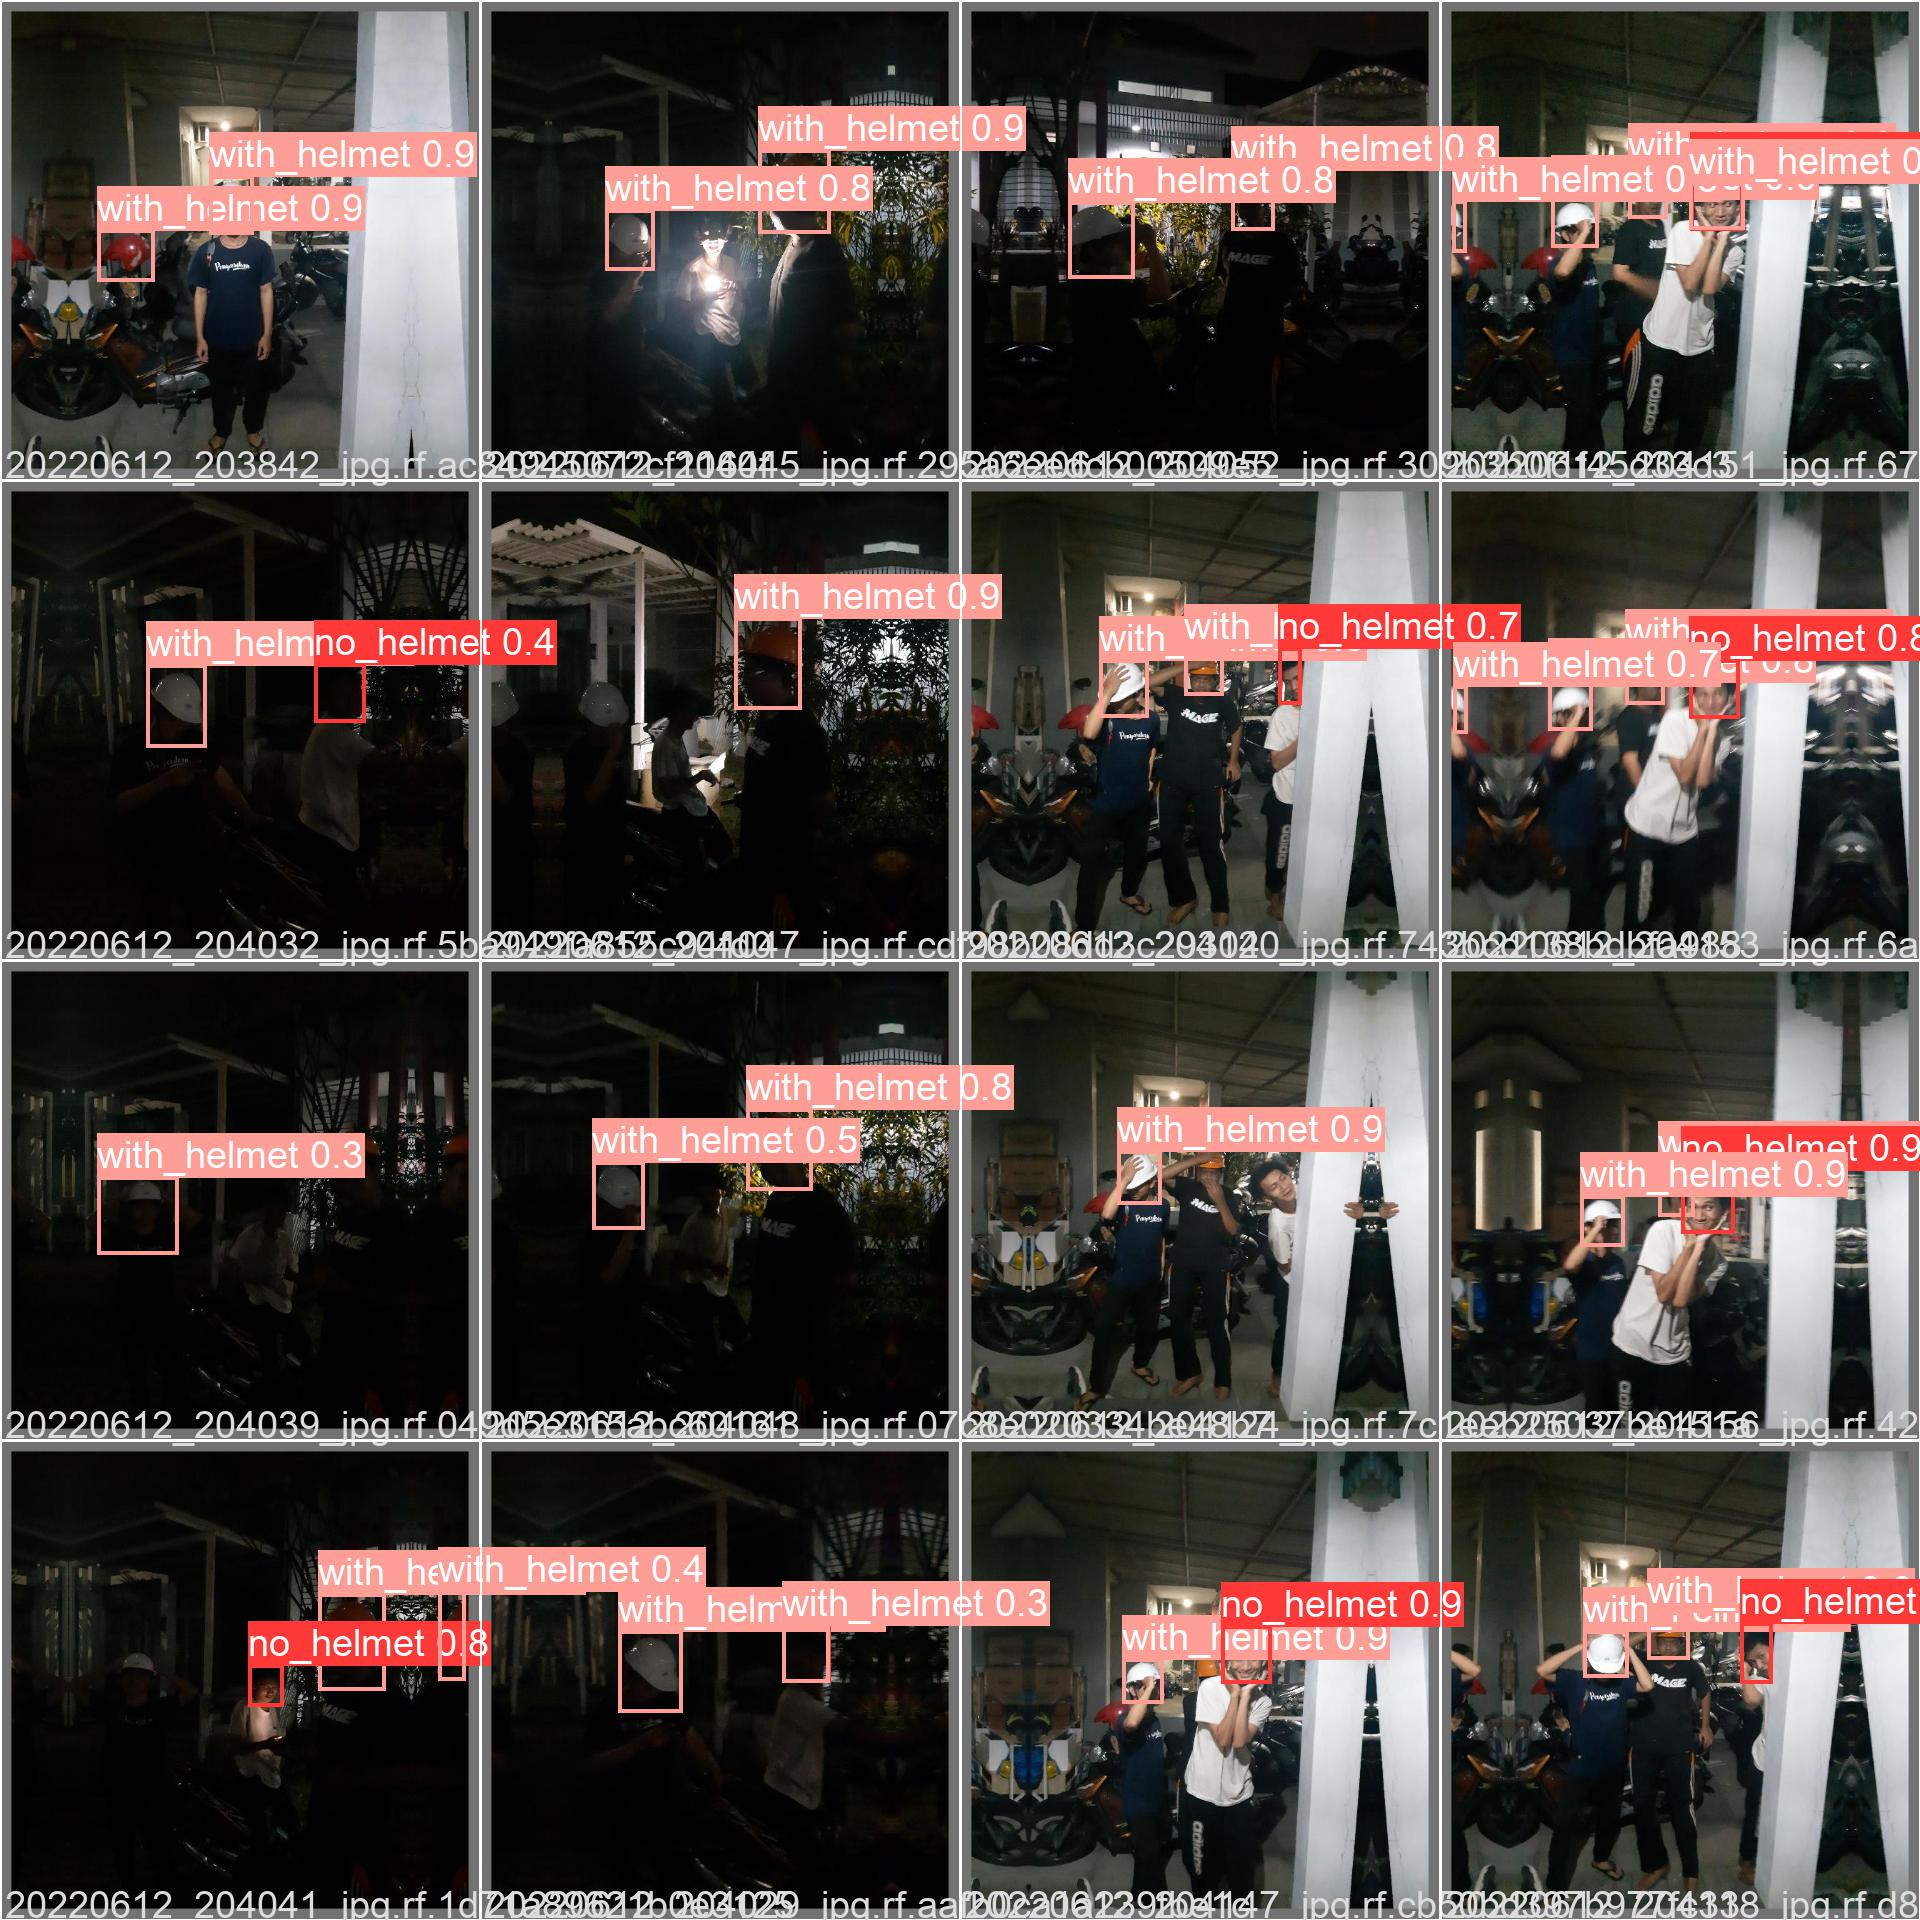
\includegraphics[scale=0.1]{gambar/train_v2_val/low_ligjt/customLarge/val_batch0_pred.jpg}
  \includegraphics[scale=0.1]{gambar/train_v2_val/low_ligjt/customLarge/val_batch0_labels.jpg}
  \caption{Hasil Prediksi dengan Anotasi Asli Pada Keadaan dengan \emph{Weight Hedec Large}}
  % \label{fig:labelbaru}  
\end{figure}